%_____________________________________________________________________________
%=============================================================================
% main.tex v8 (31-05-2015) \ldots dibuat oleh Lionov - Informatika FTIS UNPAR
% 
% Ini adalah file utama (main.tex), berisi perintah-perintah yang khusus 
% dibuat untuk template ini
%
% 			JANGAN MENGUBAH APAPUN DI DALAM FILE INI,
%			KECUALI ANDA TAHU APA YANG ANDA LAKUKAN !!!
%
% Jika ada tambahan perintah, dapat anda tuliskan di tempat yang telah disediakan 
% di baris 310 pada file ini
% Jika daftar tabel tidak digunakan, anda harus menghapus (beri komentar) secara
% manual di baris 485
%
% Bug, kritik, saran: silahkan kirimkan via email ke lionov@unpar.ac.id
%
% Perubahan pada versi 8 (31-05-2015):
%	- penambahan default data untuk beberapa keterangan dan digunakan sebagai 
%	  template dengan tanda << & >> . Data yang diubah defaultnya adalah: nama skripsi
%	  nama prodi, beserta bahasa inggrisnya.
%   - Keywords dan kata kunci di abstrak ditambahkan noindent + perbaikan lainnya
%   - Perbaikan untuk halaman tidak kosong tanpa nomor halaman romawi
%
% Perubahan pada versi sebelumnya :
%	versi 7 (27-05-2014)
%	- penambahan perintah \raggedbottom untuk menghilangkan area kosong akibat 
%	  penempatan gambar yang tidak sempurna
%	versi 6 (10-11-2013)
%	- perbaikan pada abstract dengan paragraf lebih dari satu: perbaikan vertical spacing
%	- perbaikan pada tampilan bab dan lampiran: tidak perlu menuliskan apapun untuk 
%	  menampilkan semuanya (di data.tex) atau -1 jika tidak ada lampiran
%	- halaman bernomor genap untuk halaman romawi sudah dimunculkan
%	- Kurikulum 2013 : perubahan nama buku skripsi 
%	versi 5 (21-10-2012)
%	- halaman terakhir setiap bab tidak ada headernya jika kosong
%	versi 4 (06-08-2012)
% 	- penggabungan main.tex, depan.tex dan setup.tex menjadi main.tex
% 	- menambahkan keterangan di lampiran untuk kode program 
% 	- ukuran font dapat diubah langsung di tiap lampiran
% 	versi 3 (09-07-2012): 
%	- Tidak ada di file ini
% 	versi 2 :
% 	- "Daftar Referensi" tidak perlu diubah secara manual (tidak perlu mengubah file bahasai.ldf)
% 	- Bahasa Indonesia dari abstract adalah abstrak (secara otomatis), bukan ringkasan
% 	- Spasi pada buku dokumen final adalah onehalfspacing
%
% to do : - hilangkan secara otomatis daftar tabel/gambar jika tidak digunakan
%         - (IT) aturan penulisan algoritma untuk IT (pakai algo.sty ?)
%=============================================================================

%=============================================================================
% setup.tex v2 (08-07-2012)
% Perubahan pada versi 2:
% - Menambahkan perintah untuk judulINA dan judulENG
% - Menghapus \usepackage{microtype}, yang pada beberapa kasus menjadi masalah
%=============================================================================
% depan.tex v2 (09-07-2012)
% Perubahan pada versi 2:
% - Menambahkan halaman depan dalam bahasa inggris
%=============================================================================

%setup.tex
\documentclass[11pt,a4paper,twoside,openright,notitlepage]{report} 

\usepackage[bahasa]{babel} %bahasa indonesia
\usepackage[T1]{fontenc}  %encoding
% \usepackage{mathptmx}
% \usepackage{venturisold}
% \usepackage{helvet}
% \usepackage{fouriernc} 
\usepackage{abstract} %manipulasi abstract
\usepackage{chappg} % format daftar isi 
\usepackage{color} %warna
\usepackage{etoolbox} %untuk programming if-then
\usepackage{fancyhdr} %format header & footer
\usepackage{float} %penempatan gambar di tempat yg seharusnya
\usepackage[inner=2.5cm,outer=2cm,top=2.5cm,bottom=2.5cm]{geometry} %margin
\usepackage{graphicx} %gambar
\usepackage{listings} %source code
\usepackage{lscape} %landscape untuk source code
\usepackage{multicol} %multiple column
\usepackage{ifthen} % if then
\usepackage[pagewise]{lineno} %line numbering
\usepackage{lipsum} % untuk testing
\usepackage{titlesec} %judul header
\usepackage{tocbibind} %daftar isi, gambar, tabel dll
\usepackage{tocloft} % format daftar isi 
\usepackage{setspace} %line spacing
\usepackage{xstring} %manipulasi string
\usepackage[plainpages=false,pdfpagelabels,unicode]{hyperref} %\autoref, \phantomsection & link 
\usepackage{emptypage}

\let\abstractname\Abstrak

\titleformat{\chapter}[display] {\Large\bfseries\centering}{\MakeUppercase{\chaptertitlename} \thechapter}{15pt}{\Large\MakeUppercase}

\renewcommand{\cftchapfont}{\scshape \bfseries}

\renewcommand{\cfttoctitlefont}{\hfill\Large\bfseries\MakeUppercase}
\renewcommand{\cftaftertoctitle}{\hfill}
\renewcommand{\cftloftitlefont}{\hfill\Large\bfseries\MakeUppercase}
\renewcommand{\cftafterloftitle}{\hfill}
\renewcommand{\cftlottitlefont}{\hfill\Large\bfseries\MakeUppercase}
\renewcommand{\cftafterlottitle}{\hfill}

% Tidak perlu ada kata "Bab", "Gambar" atau "Tabel" di daftar 
% \renewcommand{\cftchappresnum}{{\bf \scshape Bab} } 
% \renewcommand{\cftchapnumwidth}{1.5cm}
% \renewcommand{\cftfigpresnum}{{Gambar\ }} 
% \renewcommand{\cftfignumwidth}{2.5cm}
% \renewcommand{\cfttabpresnum}{{Tabel\ }} 
% \renewcommand{\cfttabnumwidth}{2cm}

\newcommand{\apptoc}{
	% Hapus kata "Lampiran" dari daftar isi
	%\addtocontents{toc}{\protect\renewcommand{\protect\cftchappresnum}{\bf \scshape Lampiran\  }}%
	%\addtocontents{toc}{\protect\renewcommand{\protect\cftchapnumwidth}{2.75cm}}
	\addtocontents{toc}{\protect\renewcommand{\protect\cftchappresnum}{\bf \scshape}}%	

}

\newcommand{\vnama}{Jane Doe}
\newcommand{\vlnama}{John Doe}
\newcommand{\vnpm}{1992700001}
\newcommand{\vprodiINA}{SAINS}
\newcommand{\vprodiENG}{SCIENCE}
\newcommand{\vstaINA}{UJIAN}
\newcommand{\vstaENG}{EXAM}
%\newcommand{\vjudul}{Judul Skripsi/Tugas Akhir}
\newcommand{\vpembu}{Plato}
\newcommand{\vpembs}{Euclid}
\newcommand{\vpengi}{Plato}
\newcommand{\vpengii}{Euclid}
\newcommand{\vtanggal}{1}
\newcommand{\vbulan}{Januari}
\newcommand{\vtahun}{1970}
\newcommand{\vmode}{final}
\newcommand{\vspacing}{double}
\newcommand{\vlineno}{yes}
\newcommand{\vkunciina}{Skripsi, Tugas Akhir}
\newcommand{\vkuncieng}{Undergraduate Thesis, Final Project}
\newcommand{\vkajur}{Jack Doe}
\newcommand{\vkajurmat}{Jack Doe}
\newcommand{\vkajurfis}{Jack Doe}
\newcommand{\vkajurtif}{Jack Doe}

\newcommand{\namanpm}[2]{
	\renewcommand{\vstaINA}{<<SKRIPSI/TUGAS AKHIR>>}
	\renewcommand{\vprodiINA}{<<MATEMATIKA/FISIKA/TEKNIK INFORMATIKA>>}
	\renewcommand{\vstaENG}{<<FINAL PROJECT/UNDERGRADUATE THESIS>>}
	\renewcommand{\vprodiENG}{<<MATHEMATICS/PHYSICS/INFORMATICS>>}
	\renewcommand{\vnama}{\uppercase{#1}} \renewcommand{\vlnama}{#1} \hypersetup{pdfauthor={#2 - #1}}
	\renewcommand{\vnpm}{#2} \hypersetup{pdfcreator={#2}} \StrChar{\vnpm}{6}[\vprodiN]
	\ifdefstring{\vprodiN}{1}{
		\renewcommand{\vprodiINA}{MATEMATIKA} \renewcommand{\vprodiENG}{MATHEMATICS} 
		\renewcommand{\vstaINA}{SKRIPSI} \renewcommand{\vstaENG}{FINAL PROJECT} \renewcommand{\vkajur}{\vkajurmat}}{}
	\ifdefstring{\vprodiN}{2}{
		\renewcommand{\vprodiINA}{FISIKA} \renewcommand{\vprodiENG}{PHYSICS} 
		\renewcommand{\vstaINA}{SKRIPSI} \renewcommand{\vstaENG}{FINAL PROJECT} \renewcommand{\vkajur}{\vkajurfis}}{}
	\ifdefstring{\vprodiN}{3}{
		\renewcommand{\vprodiINA}{TEKNIK INFORMATIKA} \renewcommand{\vprodiENG}{INFORMATICS} 
		\renewcommand{\vstaINA}{SKRIPSI} \renewcommand{\vstaENG}{UNDERGRADUATE THESIS} \renewcommand{\vkajur}{\vkajurtif}}{}}

%\newcommand{\judul}[1]{\renewcommand{\vjudul}{\uppercase{#1}}\hypersetup{pdftitle={#1}, pdfsubject={#1}}}
\newcommand{\pembimbing}[2]{\renewcommand{\vpembu}{#1}\renewcommand{\vpembs}{#2}}
\newcommand{\penguji}[2]{\renewcommand{\vpengi}{#1}\renewcommand{\vpengii}{#2}}
\newcommand{\kajur}[3]{\renewcommand{\vkajurmat}{#1}\renewcommand{\vkajurfis}{#2}\renewcommand{\vkajurtif}{#3}}
\renewcommand{\vbulan}{<<bulan>>}
\newcommand{\tanggal}[3]{\renewcommand{\vtanggal}{#1}\renewcommand{\vtahun}{#3}
	\newcommand{\vcbulan}{#2}
	\ifdefstring{\vcbulan}{1}{\renewcommand{\vbulan}{Januari}}{}
	\ifdefstring{\vcbulan}{2}{\renewcommand{\vbulan}{Februari}}{}
	\ifdefstring{\vcbulan}{3}{\renewcommand{\vbulan}{Maret}}{}
	\ifdefstring{\vcbulan}{4}{\renewcommand{\vbulan}{April}}{}
	\ifdefstring{\vcbulan}{5}{\renewcommand{\vbulan}{Mei}}{}
	\ifdefstring{\vcbulan}{6}{\renewcommand{\vbulan}{Juni}}{}
	\ifdefstring{\vcbulan}{7}{\renewcommand{\vbulan}{Juli}}{}
	\ifdefstring{\vcbulan}{8}{\renewcommand{\vbulan}{Agustus}}{}
	\ifdefstring{\vcbulan}{9}{\renewcommand{\vbulan}{September}}{}
	\ifdefstring{\vcbulan}{10}{\renewcommand{\vbulan}{Oktober}}{}
	\ifdefstring{\vcbulan}{11}{\renewcommand{\vbulan}{November}}{}
	\ifdefstring{\vcbulan}{12}{\renewcommand{\vbulan}{Desember}}{}	
}

\newcommand{\judulINA}[1]{\newcommand{\vjudulINA}{\uppercase{#1}}\hypersetup{pdftitle={#1},pdfsubject={#1}}}
\newcommand{\judulENG}[1]{\newcommand{\vjudulENG}{\uppercase{#1}}\hypersetup{pdftitle={#1},pdfsubject={#1}}}
\newcommand{\abstrakINA}[1]{\newcommand{\vabstrakina}{#1}}
\newcommand{\abstrakENG}[1]{\newcommand{\vabstrakeng}{#1}}
\newcommand{\kunciINA}[1]{\renewcommand{\vkunciina}{#1} \hypersetup{pdfkeywords={#1}}}
\newcommand{\kunciENG}[1]{\renewcommand{\vkuncieng}{#1}}
\newcommand{\untuk}[1]{\newcommand{\vuntuk}{#1}}
\newcommand{\prakata}[1]{\newcommand{\vprakata}{#1}}
\newcommand{\mode}[1]{\renewcommand{\vmode}{#1}}
\newcommand{\linespacing}[1]{\renewcommand{\vspacing}{#1}}
\newcommand{\linenumber}[1]{\renewcommand{\vlineno}{#1}}

\newcommand{\bab}[1]{\newcommand{\vbab}{#1}}
\newcommand{\lampiran}[1]{\renewcommand{\vlmp}{#1}}

\newcommand{\vpilbab}{0}
\newcommand{\vbaba}{0}\newcommand{\vbabb}{0}\newcommand{\vbabc}{0}
\newcommand{\vbabd}{0}\newcommand{\vbabe}{0}\newcommand{\vbabf}{0}
\newcommand{\vbabg}{0}\newcommand{\vbabh}{0}\newcommand{\vbabi}{0}
\newcommand{\vpillmp}{0}
\newcommand{\vlmpa}{0}\newcommand{\vlmpb}{0}\newcommand{\vlmpc}{0}
\newcommand{\vlmpd}{0}\newcommand{\vlmpe}{0}\newcommand{\vlmpf}{0}
\newcommand{\vlmpg}{0}\newcommand{\vlmph}{0}\newcommand{\vlmpi}{0}
\newcommand{\vlmp}{x}

%	\ifdefempty{#1}{\bab{1,2,3,4,5,6,7,8,9} \tampilbab{\vbab}}{
\newcommand{\tampilbab}[1]{
	\ifdefempty{#1}{
		\renewcommand{\vbaba}{1}\renewcommand{\vbabb}{1}\renewcommand{\vbabc}{1}
		\renewcommand{\vbabd}{1}\renewcommand{\vbabe}{1}\renewcommand{\vbabf}{1}
		\renewcommand{\vbabg}{1}\renewcommand{\vbabh}{1}\renewcommand{\vbabi}{1}}{
	\renewcommand{\do}[1]{
		\renewcommand{\vpilbab}{##1}
		\ifdefstring{\vpilbab}{1}{\renewcommand{\vbaba}{1}}{}
		\ifdefstring{\vpilbab}{2}{\renewcommand{\vbabb}{1}}{}
		\ifdefstring{\vpilbab}{3}{\renewcommand{\vbabc}{1}}{}
		\ifdefstring{\vpilbab}{4}{\renewcommand{\vbabd}{1}}{}
		\ifdefstring{\vpilbab}{5}{\renewcommand{\vbabe}{1}}{}
		\ifdefstring{\vpilbab}{6}{\renewcommand{\vbabf}{1}}{}
		\ifdefstring{\vpilbab}{7}{\renewcommand{\vbabg}{1}}{}
		\ifdefstring{\vpilbab}{8}{\renewcommand{\vbabh}{1}}{}
		\ifdefstring{\vpilbab}{9}{\renewcommand{\vbabi}{1}}{}
	}
	\expandafter\docsvlist\expandafter{#1}
	}
}

\newcommand{\tampillmp}[1]{
	\ifdefempty{#1}{
		\renewcommand{\vlmpa}{1}\renewcommand{\vlmpb}{1}\renewcommand{\vlmpc}{1}
		\renewcommand{\vlmpd}{1}\renewcommand{\vlmpe}{1}\renewcommand{\vlmpf}{1}
		\renewcommand{\vlmpg}{1}\renewcommand{\vlmph}{1}\renewcommand{\vlmpi}{1}}{
	\ifdefstring{#1}{-1}{ }{
		\renewcommand{\do}[1]{ 
			\renewcommand{\vpillmp}{##1}
			\ifdefstring{\vpillmp}{A}{\renewcommand{\vlmpa}{1}}{}
			\ifdefstring{\vpillmp}{B}{\renewcommand{\vlmpb}{1}}{}
			\ifdefstring{\vpillmp}{C}{\renewcommand{\vlmpc}{1}}{}
			\ifdefstring{\vpillmp}{D}{\renewcommand{\vlmpd}{1}}{}
			\ifdefstring{\vpillmp}{E}{\renewcommand{\vlmpe}{1}}{}
			\ifdefstring{\vpillmp}{F}{\renewcommand{\vlmpf}{1}}{}
			\ifdefstring{\vpillmp}{G}{\renewcommand{\vlmpg}{1}}{}
			\ifdefstring{\vpillmp}{H}{\renewcommand{\vlmph}{1}}{}
			\ifdefstring{\vpillmp}{I}{\renewcommand{\vlmpi}{1}}{}}
		}
	\expandafter\docsvlist\expandafter{#1}
	}
}

\newcommand{\appspacing}{
	\ifdefstring{\vspacing}{single}{\singlespacing}{}
	\ifdefstring{\vspacing}{onehalf}{\onehalfspacing}{}
	\ifdefstring{\vspacing}{double}{\doublespacing}{}
	\ifdefstring{\vmode}{final}{\onehalfspacing}{}
}

\newcommand{\appline}{
	\ifdefstring{\vmode}{final}{\renewcommand{\vlineno}{no}}{}
	\ifdefstring{\vlineno}{yes}{\linenumbers \def\linenumberfont{\normalfont\tiny\sffamily}}{}
	\ifdefstring{\vlineno}{no}{\lstset{numbers=left, stepnumber=1, numbersep=5pt}}{}
	
}

\newcommand{\appmargin}{
	\ifdefstring{\vmode}{final}{}{\newgeometry{inner=3cm,outer=2.75cm,top=2cm,bottom=2cm}}
}

\renewcommand{\abstractnamefont}{\bf \MakeUppercase}

\makeatletter
\def\headrule{{%
  \if@fancyplain\let\headrulewidth\plainheadrulewidth\fi
  \hrule\@height\footrulewidth\@width\headwidth\vskip2pt%
  \hrule\@height\headrulewidth\@width\headwidth\vskip-\headrulewidth\vskip-4pt
}}
\def\footrule{}

\def\cleardoublepage{
	\clearpage
	\if@twoside \ifodd\c@page
	\else
		\hbox{}
		\vspace{\fill}
		\thispagestyle{empty}
		\newpage
	\if@twocolumn\hbox{}\newpage\fi\fi\fi}
\makeatother

\renewcommand{\headrulewidth}{1.25pt}
\renewcommand{\footrulewidth}{0.25pt}

\setlength{\headheight}{15pt}
\fancyhead[LE,RO]{\thepage}
\fancyhead[RE]{\small{\textsc{\nouppercase{\leftmark}}}}
\fancyhead[LO]{\small{\textsc{\nouppercase{\rightmark}}}}
\fancyfoot{}

\hypersetup{unicode=true,colorlinks=true,linkcolor=blue,citecolor=green,filecolor=magenta, urlcolor=cyan}

\lstset{basicstyle=\tiny, commentstyle=\color{blue}}
\lstset{frame=leftline, tabsize=4, breaklines=true}

%=============================================================================

%tambahkan perintah yang anda butuhkan di sini :

%=============================================================================
%end setup.tex

%_____________________________________________________________________________
%=============================================================================
% data.tex v8 (02-10-2016) \ldots dibuat oleh Lionov - Informatika FTIS UNPAR
%
% Perubahan pada versi 8 (02-10-2016)
%	- Perubahan keterangan pada spacing: Otomatis spasi 1 untuk buku skripsi 
%	  final dan 1.5 untuk buku sidang
%	- Penggunaan kantlipsum
%_____________________________________________________________________________
%=============================================================================

%=============================================================================
% 								PETUNJUK
%=============================================================================
% Ini adalah file data (data.tex)
% Masukkan ke dalam file ini, data-data yang diperlukan oleh template ini
% Cara memasukkan data dijelaskan di setiap bagian
% Data yang WAJIB dan HARUS diisi dengan baik dan benar adalah SELURUHNYA !!
% Hilangkan tanda << dan >> jika anda menemukannya
%=============================================================================

%_____________________________________________________________________________
%=============================================================================
% 								BAGIAN 0
%=============================================================================
% PERHATIAN!! PERHATIAN!! Bagian ini hanya ada untuk sementara saja
% Jika "DAFTAR ISI" tidak bisa berada di bagian tengah halaman, isi dengan XXX
% jika sudah benar posisinya, biarkan kosong (i.e. \daftarIsiError{ })
%=============================================================================
\daftarIsiError{ }
%=============================================================================

%_____________________________________________________________________________
%=============================================================================
% 								BAGIAN I
%=============================================================================
% Tambahkan package2 lain yang anda butuhkan di sini
%=============================================================================
\usepackage{booktabs} 
\usepackage[table]{xcolor}
\usepackage{longtable}
\usepackage{amssymb}
\usepackage{todo}
\usepackage{verbatim} 		%multilne comment
\usepackage{pgfplots}
%=============================================================================

%_____________________________________________________________________________
%=============================================================================
% 								BAGIAN II
%=============================================================================
% Mode dokumen: menetukan halaman depan dari dokumen, apakah harus mengandung 
% prakata/pernyataan/abstrak dll (termasuk daftar gambar/tabel/isi) ?
% - kosong : tidak ada halaman depan sama sekali (untuk dokumen yang 
%            dipergunakan pada proses bimbingan)
% - cover : cover saja tanpa daftar isi, gambar dan tabel
% - sidang : cover, daftar isi, gambar, tabel 
% - sidang_akhir : mode sidang + abstrak + abstract
% - final : seluruh halaman awal dokumen (untuk cetak final)
% Jika tidak ingin mencetak daftar tabel/gambar (misalkan karena tidak ada 
% isinya), edit manual di baris 439 dan 440 pada file main.tex
%=============================================================================
% \mode{kosong}
% \mode{cover}
% \mode{sidang}
\mode{sidang_akhir}
% \mode{final} 
%=============================================================================

%_____________________________________________________________________________
%=============================================================================
% 								BAGIAN III
%=============================================================================
% Line numbering: penomoran setiap baris, otomatis di-reset setiap berganti
% halaman
% - yes: setiap baris diberi nomor
% - no : baris tidak diberi nomor, otomatis untuk mode final
%=============================================================================
\linenumber{yes}
%=============================================================================

%_____________________________________________________________________________
%=============================================================================
% 								BAGIAN IV
%=============================================================================
% Linespacing: jarak antara baris 
% - single	: wajib (dan otomatis jika ingin mencetak buku skripsi, opsi yang 
%			  disediakan untuk bimbingan, jika pembimbing tidak keberatan 
%			  (untuk menghemat kertas)
% - onehalf	: default dan wajib (dan otomatis) jika ingin mencetak dokumen
%             untuk sidang.
% - double 	: jarak yang lebih lebar lagi, jika pembimbing berniat memberi 
%             catatan yg banyak di antara baris (dianjurkan untuk bimbingan)
%=============================================================================
\linespacing{single}
%\linespacing{onehalf}
%\linespacing{double}
%=============================================================================

%_____________________________________________________________________________
%=============================================================================
% 								BAGIAN V
%=============================================================================
% Tidak semua skripsi memuat gambar dan/atau tabel. Untuk skripsi yang seperti
% itu, tidak diperlukan Daftar Gambar dan Daftar Tabel. Sayangnya hal ini 
% sulit dilakukan secara manual karena membutuhkan kedisiplinan pengguna 
% template.  
% Jika tidak akan menampilkan Daftar Gambar/Tabel, isi dengan NO. Jika ingin
% menampilkan, kosongkan parameter (i.e. \gambar{ }, \tabel{ })
%=============================================================================
\gambar{ }
\tabel{ }
%=============================================================================

%_____________________________________________________________________________
%=============================================================================
% 								BAGIAN VI
%=============================================================================
% Bab yang akan dicetak: isi dengan angka 1,2,3 s.d 9, sehingga bisa digunakan
% untuk mencetak hanya 1 atau beberapa bab saja
% Jika lebih dari 1 bab, pisahkan dengan ',', bab akan dicetak terurut sesuai 
% urutan bab (e.g. \bab{1,2,3}).
% Untuk mencetak seluruh bab, kosongkan parameter (i.e. \bab{ })  
% Catatan: Jika ingin menambahkan bab ke-10 dan seterusnya, harus dilakukan 
% secara manual
%=============================================================================
\bab{ }
%=============================================================================

%_____________________________________________________________________________
%=============================================================================
% 								BAGIAN VII
%=============================================================================
% Lampiran yang akan dicetak: isi dengan huruf A,B,C s.d I, sehingga bisa 
% digunakan untuk mencetak hanya 1 atau beberapa lampiran saja
% Jika lebih dari 1 lampiran, pisahkan dengan ',', lampiran akan dicetak 
% terurut sesuai urutan lampiran (e.g. \bab{A,B,C}).
% Jika tidak ingin mencetak lampiran apapun, isi dengan -1 (i.e. \lampiran{-1})
% Untuk mencetak seluruh mapiran, kosongkan parameter (i.e. \lampiran{ })  
% Catatan: Jika ingin menambahkan lampiran ke-J dan seterusnya, harus 
% dilakukan secara manual
%=============================================================================
\lampiran{ }
%=============================================================================

%_____________________________________________________________________________
%=============================================================================
% 								BAGIAN VIII
%=============================================================================
% Data diri dan skripsi/tugas akhir
% - namanpm: Nama dan NPM anda, penggunaan huruf besar untuk nama harus benar
%			 dan gunakan 10 digit npm UNPAR, PASTIKAN BAHWA BENAR !!!
%			 (e.g. \namanpm{Jane Doe}{1992710001}
% - judul : Dalam bahasa Indonesia, perhatikan penggunaan huruf besar, judul
%			tidak menggunakan huruf besar seluruhnya !!! 
% - tanggal : isi dengan {tangga}{bulan}{tahun} dalam angka numerik, jangan 
%			  menuliskan kata (e.g. AGUSTUS) dalam isian bulan
%			  Tanggal ini adalah tanggal dimana anda akan melaksanakan sidang 
%			  ujian akhir skripsi/tugas akhir
% - pembimbing: isi dengan pembimbing anda, lihat daftar dosen di file dosen.tex
%				jika pembimbing hanya 1, kosongkan parameter kedua 
%				(e.g. \pembimbing{\JND}{  } ) , \JND adalah kode dosen
% - penguji : isi dengan para penguji anda, lihat daftar dosen di file dosen.tex
%				(e.g. \penguji{\JHD}{\JCD} ) , \JND dan \JCD adalah kode dosen
% !!Lihat singkatan pembimbing dan penguji anda di file dosen.tex
%=============================================================================
\namanpm{Billy Yanuar}{2012730017}	%hilangkan tanda << & >>
\tanggal{<<tanggal>>}{<<bulan>>}{2017}			%hilangkan tanda << & >>
\pembimbing{<<pembimbing1>>}{<<pembimbing2>>} %hilangkan tanda << & >>    
\penguji{<<penguji 1>>}{<<penguji 2>>} 				%hilangkan tanda << & >>
%=============================================================================

%_____________________________________________________________________________
%=============================================================================
% 								BAGIAN IX
%=============================================================================
% Judul dan title : judul bhs indonesia dan inggris
% - judulINA: judul dalam bahasa indonesia
% - judulENG: title in english
% PERHATIAN: - langsung mulai setelah '{' awal, jangan mulai menulis di baris 
%			   bawahnya
%			 - Gunakan \texorpdfstring{\\}{} untuk pindah ke baris baru
%			 - Judul TIDAK ditulis dengan menggunakan huruf besar seluruhnya !!
%			 - Gunakan perintah \texorpdfstring{\\}{} untuk baris baru
%=============================================================================
\judulINA{Sistem Penilaian Sidang Skripsi 2 dengan AngularJS}
\judulENG{The Thesis 2 Assessment Defense System}
%_____________________________________________________________________________
%=============================================================================
% 								BAGIAN X
%=============================================================================
% Abstrak dan abstract : abstrak bhs indonesia dan inggris
% - abstrakINA: abstrak bahasa indonesia
% - abstrakENG: abstract in english
% PERHATIAN: langsung mulai setelah '{' awal, jangan mulai menulis di baris 
%			 bawahnya
%=============================================================================
\abstrakINA{Mata kuliah Skripsi 2 merupakan salah satu syarat wajib dalam proses pembelajaran yang dilakukan di Program Studi Teknik Informatika Universitas Katolik Parahyangan, Bandung. Sistem kini yang diterapkan untuk melakukan penilaian pada sidang Skripsi 2 masih menggunakan kertas penilaian, dimana penilai akan menuliskan nilai yang diinginkan lalu melakukan perhitungan dengan alat hitung masing-masing untuk mendapatkan nilai akhir mahasiswa. Untuk itu, dibuatlah Sistem Penilaian Sidang Skripsi 2 yang berupa situs \textit{web} yang membantu perhitungan dan penyimpanan nilai sidang mata kuliah Skripsi 2 tersebut. Sistem Penilaian Sidang Skripsi 2 dibuat menggunakan bahasa PHP yang diintegrasikan dengan AngularJS sehingga dapat melakukan otomatisasi perhitungan nilai akhir mahasiswa.\\
AngularJS merupakan \textit{framework} yang dipakai dalam pembangunan \textit{single page application}. Kemudahan pemakaian AngularJS merupakan salah satu nilai tambah tersendiri. AngularJS memiliki konsep MVC (\textit{Model, View, Controller}) yang bekerja secara \textit{front-end} (di bagian \textit{layout web}) sehingga dapat diintegrasikan oleh \textit{framework} lain, seperti \textit{codeigniter}.\\
Pengujian Sistem Penilaian Sidang Skripsi 2 dilakukan dengan membandingkan hasil perhitungan nilai akhir mahasiswa dari 5 sidang skripsi 2 yang berlangsung pada Semester Ganjil 2016/2017. Pengujian tersebut dilakukan dengan cara membandingkan hasil perhitungan dari Sistem Penilaian Sidang Skripsi 2 dan dari sistem kini. Dari hasil pengujian tersebut, didapatkan bahwa perhitungan yang dilakukan oleh sistem usulan lebih akurat dibandingkan dengan sistem kini.}
\abstrakENG{One of the graduate condition in Informatics Engineering Parahyangan Catholic University, Bandung is Thesis 2 courses. The current system applied for assessment in defense of the Thesis 2 is still using scoring paper, where the assessor will write down the desired value and the perform the calculation with the calculator to get the final grade. Therefore, The Thesis 2 Assessment Defense System was created in a website that helped the calculation and store the final grade of Thesis 2 defense. The Thesis 2 Assessment Defense System was built in PHP programming language which is integrated with AngularJS so it can perform automatic calculation of the final grade.\\
AngularJS is a framework that used in single page application. Ease of use is one of its special advantage. AngularJS's concept is MVC (Model, View, Controller) that works on front-end (in layout web) so it can be integrated with other framework such as codeigniter.\\
The Thesis 2 Assessment Defense System testing is done by comparing the calculation result of The Thesis 2 Assessment Defense System and the current system used. From the test result, we obtained that the calculation of The Thesis 2 Assessment Defense System is more accurate than the current system used.
} 
%=============================================================================

%_____________________________________________________________________________
%=============================================================================
% 								BAGIAN XI
%=============================================================================
% Kata-kata kunci dan keywords : diletakkan di bawah abstrak (ina dan eng)
% - kunciINA: kata-kata kunci dalam bahasa indonesia
% - kunciENG: keywords in english
%=============================================================================
\kunciINA{Sistem Penilaian Skripsi 2, PHP, AngularJS}
\kunciENG{The Thesis 2 Assessment Defense System, PHP, AngularJS}
%=============================================================================

%_____________________________________________________________________________
%=============================================================================
% 								BAGIAN XII
%=============================================================================
% Persembahan : kepada siapa anda mempersembahkan skripsi ini ...
%=============================================================================
\untuk{Teknik Informatika UNPAR, diri sendiri}
%=============================================================================

%_____________________________________________________________________________
%=============================================================================
% 								BAGIAN XIII
%=============================================================================
% Kata Pengantar: tempat anda menuliskan kata pengantar dan ucapan terima 
% kasih kepada yang telah membantu anda bla bla bla ....  
%=============================================================================
\prakata{Puji syukur kepada Tuhan Yang Maha Esa atas berkat dan yang diberikan kepada penulis sehingga dapat menyelesaikan tugas akhir dengan judul \textbf{Sistem Penilaian Sidang Skripsi 2 dengan Angular JS}  dengan baik dan tepat waktu. Penulis juga berterima kasih kepada pihak-pihak yang telah memberikan dukungan dan bantuan kepada penulis dalam menyelesaikan tugas akhir ini, yaitu: 
	\begin{enumerate}
		\item Keluarga dan teman-teman yang selalu memberikan dukungan dan semangat kepada penulis. 
		\item Bapak Pascal Alfadian sebagai dosen pembimbing yang telah membimbing penulis hingga dapat menyelesaikan tugas akhir ini.
		\item Pihak-pihak lain yang belum disebutkan, yang berperan dalam penyelesaian tugas akhir ini. 
	\end{enumerate}
	
	Akhir kata, penulis berharap agar tugas akhir ini dapat bermanfaat bagi pembaca yang hendak melakukan penelitian dan pengembangan yang terkait dengan tugas akhir ini.
}
%=============================================================================

%_____________________________________________________________________________
%=============================================================================
% 								BAGIAN XIV
%=============================================================================
% Tambahkan hyphen (pemenggalan kata) yang anda butuhkan di sini 
%=============================================================================
\hyphenation{ma-te-ma-ti-ka}
\hyphenation{fi-si-ka}
\hyphenation{tek-nik}
\hyphenation{in-for-ma-ti-ka}
%=============================================================================

%_____________________________________________________________________________
%=============================================================================
% 								BAGIAN XV
%=============================================================================
% Tambahkan perintah yang anda buat sendiri di sini 
%=============================================================================
\newcommand{\vtemplateauthor}{lionov}
\pgfplotsset{compat=newest}
\usetikzlibrary{patterns}
%=============================================================================

% Copyright \textcopyright [Lionov] [09-10-2016]. All rights reserved
%_____________________________________________________________________________
%=============================================================================
% dosen.tex v6 (19-08-2016) \ldots dibuat oleh Lionov - Informatika FTIS UNPAR
%
% Perubahan pada versi 6 (19-08-2016)
% 	- Penambahan dosen (Farica, Claudio).
%	- Penghapusan dosen (Oerip)
% 	- Perubahan singkatan untuk dosen Informatika sesuai ketentuan prodi
%	- Perbaikan "catatan untuk mhs teknik informatika"
%
% Perubahan pada versi sebelumnya dapat dilihat di bagian akhir file ini
%_____________________________________________________________________________
%=============================================================================

%=============================================================================
% Data dosen dan kajur FTIS - JANGAN MENGUBAH APAPUN DI BAGIAN INI, KECUALI
% untuk mengubah kajur (jika kajur telah berganti orang) atau menambahkan 
% pembimbing anda yang tidak/belum tercantum pada daftar ini atau 
% memperbaiki penulisan gelar jika penguji anda meminta
% perintah: \kajur{1}{2}{3} 1: Matematika 2: Fisika 3: Teknik Informatika
%=============================================================================
% CATATAN UNTUK MAHASISWA TEKNIK INFORMATIKA :
% dosen yang ditandai * :
% - jika menjadi pembimbing : harus diganti, penggantinya mengikuti petunjuk
% 	dari koordinator Skripsi !
% - jika menjadi penguji: tidak diganti, tetapi hapus komentar (tanda % dan *) 
%	agar dapat digunakan
%=============================================================================

\kajur{\JDL}{\PNG}{\MTA} 

%dummy person
\newcommand{\JND}{Jane\,Doe} 
\newcommand{\JHD}{John\,Doe}
\newcommand{\JCD}{Jack\,Doe}

% Dosen-dosen Program Studi Matematika
\newcommand{\JDL}{Dr.\,Julius\,Dharma\,Lesmono}
\newcommand{\FAR}{Farah\,Kristiani,\,M.Si.}
\newcommand{\ERW}{Erwinna\,Chendra,\,M.Si.}
\newcommand{\FJP}{Dr.\,Ferry\,Jaya\,Permana,\,ASAI}
\newcommand{\AGS}{Agus\,Sukmana,\,M.Sc.}
\newcommand{\WSB}{Prof.\,M.\,Wono\,Setya\,Budhi,\,Ph.D.}
\newcommand{\LIM}{Liem\,Chin,\,M.Si.}
\newcommand{\IWS}{Iwan\,Sugiarto,\,M.Si.}
\newcommand{\IVM}{Ivonne\,Martin,\,M.Sc.}
\newcommand{\OWN}{Livia\,Owen,\,M.Si.}
\newcommand{\BNY}{Benny\,Yong,\,M.Si.}
\newcommand{\TFK}{Taufik\,Limansyah,\,M.T.}
\newcommand{\MRA}{Maria\,Anestasia,\,M.Si.}

% Dosen-dosen Program Studi Fisika
\newcommand{\PCT}{Paulus\,Cahyono\,Tjiang,\,Ph.D.}
\newcommand{\BSB}{Prof.\,B.\,Suprapto\,Brotosiswojo,\,Ph.D.}
\newcommand{\RUS}{Aloysius\,Rusli,\,Ph.D.}
\newcommand{\KMG}{Kian\,Ming,\,M.Si.}
\newcommand{\SHS}{Sylvia\,Hastuti\,Sutanto,\,Ph.D.}
\newcommand{\JVS}{Janto\,Vincent\,Sulungbudi,\,S.Si.}
\newcommand{\FLA}{Flaviana,\,M.T.}
\newcommand{\PNG}{Philips\,Nicolas\,Gunawidjaja,\,Ph.D.}
\newcommand{\ELK}{Elok\,Fidiani,\,M.Sc.}
\newcommand{\RIS}{Risti\,Suryantari,\,M.Sc.}
\newcommand{\HAS}{Haryanto\,Siahaan,\,Ph.D.}
\newcommand{\RND}{Reinard\,Primulando,\,Ph.D.}
\newcommand{\FEY}{Farica\,Edgina\,Yosafat,\,M.Si.}
 
% Dosen-dosen Program Studi Teknik Informatika
\newcommand{\CEN}{Dr.rer.nat.\,Cecilia\,Esti\,Nugraheni}
\newcommand{\VSM}{Dr.\,Veronica\,Sri\,Moertini}
\newcommand{\RDL}{Rosa\,De\,Lima,\,M.Kom.}
\newcommand{\TAB}{Dott.\,Thomas\,Anung\,Basuki}
\newcommand{\LNV}{Lionov,\,M.Sc.}
\newcommand{\MTA}{Mariskha\,Tri\,Adithia,\,P.D.Eng}
\newcommand{\LCA}{Luciana\,Abednego,\,M.T.}
\newcommand{\ELH}{Elisati\,Hulu,\,M.T.}
% * \newcommand{\CHW}{Chandra\,Wijaya,\,M.T.}
\newcommand{\GDK}{Gede\,Karya,\,M.T.,\,CISA}
\newcommand{\NIS}{Nico\,Saputro,\,M.T.}
% * \newcommand{\JNH}{Joanna\,Helga,\,M.Sc.}
% * \newcommand{\PAN}{Pascal\,Alfadian,\,M.Comp.} 
% * \newcommand{\HUH}{Husnul\,Hakim,\,M.T.} 
% * \newcommand{\VAN}{Vania\,Natali,\,M.T.} 
% * \newcommand{\ABS}{Aditya\,Bagoes\,Saputra,\,M.T.} 
% * \newcommand{\CLF}{Claudio\,Franciscus,\,M.T.} 
% * \newcommand{\NAT}{Natalia,\,M.Si.} 

% Copyright \textcopyright [Lionov] [09-10-2016]. All rights reserved

\begin{document}

\raggedbottom

\def\bibname{Daftar Referensi}
\def\abstractname{Abstrak}

\pagestyle{empty}

%depan.tex
\ifdefstring{\vmode}{kosong}{}{

\pagenumbering{roman}

%cover INA
\begin{center}
	{\Large\bf \vstaINA \\} 	\vspace{1.5cm}
	{\Large \bf \vjudulINA \\} \vspace{2.5cm}
	\includegraphics[scale=0.4]{Gambar/logo-unpar}\\ \vspace{1cm}
	{\Large \bf \vnama \\} \vspace{0.5cm}
	{\Large \bf NPM: \vnpm \\}
	\vfill
	\Large{ \textbf { 
		PROGRAM STUDI \vprodiINA \\
		FAKULTAS TEKNOLOGI INFORMASI DAN SAINS\\
		UNIVERSITAS KATOLIK PARAHYANGAN\\
		\vtahun 
	}}
\end{center}
\cleardoublepage

%cover ENG
\begin{center}
	{\Large\bf \vstaENG \\} 	\vspace{1.5cm}
	{\Large \bf \vjudulENG \\} \vspace{2.5cm}
	\includegraphics[scale=0.4]{Gambar/logo-unpar}\\ \vspace{1cm}
	{\Large \bf \vnama \\} \vspace{0.5cm}
	{\Large \bf NPM: \vnpm \\}
	\vfill
	\Large{ \textbf { 
		DEPARTMENT OF \vprodiENG \\
		FACULTY OF INFORMATION TECHNOLOGY AND SCIENCES\\
		PARAHYANGAN CATHOLIC UNIVERSITY\\
		\vtahun 
	}}
\end{center}
\cleardoublepage


% Lembar pengesahan
\ifdefstring{\vmode}{final}{
\begin{center}
	{\Large\bf LEMBAR PENGESAHAN \\} 	\vspace{1.5cm}
	{\Large \bf \vjudulINA \\} 			\vspace{1cm}
	{\Large \bf \vnama \\}				\vspace{0.5cm}
	{\Large \bf NPM: \vnpm \\}			\vspace{1.5cm}
	\large{ \bfseries{
		\begin{centering} 
			Bandung, \vtanggal\ \vbulan\ \vtahun \\ \vspace{0.25cm} Menyetujui,\\
			\vspace{0.75cm}
			\ifdefempty{\vpembs}
					{\centering Pembimbing Tunggal\\ \vspace{2cm} \vpembu\\}
					{ 	\begin{minipage}[b]{0.46\linewidth}
							\centering Pembimbing Utama \\ \vspace{2.25cm} \vpembu \\
						\end{minipage} \hspace{0.5cm}
						\begin{minipage}[b]{0.46\linewidth}
							\centering Pembimbing Pendamping \\	\vspace{2.25cm} \vpembs \\
						\end{minipage}	
					}
		\end{centering}
		\vspace{1.25cm}
		\begin{centering}	
			\begin{minipage}[b]{0.46\linewidth}
				\centering Ketua Tim Penguji \\ \vspace{2.25cm} \vpengi \\
			\end{minipage} \hspace{0.5cm}
			\begin{minipage}[b]{0.46\linewidth}
				\centering Anggota Tim Penguji \\ \vspace{2.25cm} \vpengii 
			\end{minipage}
		\end{centering}
		\vspace{1.5cm} \\
		\centering Mengetahui,\\ \vspace{0.5cm}	
		Ketua Program Studi \\ \vspace{2.25cm} \vkajur\\
	}}			
\end{center}
\cleardoublepage

% Lembar Pernyataan
\vspace*{4cm}
{\Large\bf \centering PERNYATAAN\\} \vspace{1cm}
\noindent
Dengan ini saya yang bertandatangan di bawah ini menyatakan bahwa \MakeLowercase{\vstaINA} dengan judul:  \vspace{0.5cm}
\begin{center}
	{\large \bf \vjudulINA \\}
\end{center}
\vspace{0.75cm}
adalah benar-benar karya saya sendiri, dan saya tidak melakukan penjiplakan atau pengutipan dengan cara-cara yang tidak sesuai dengan etika keilmuan yang berlaku dalam masyarakat keilmuan.
			
Atas pernyataan ini, saya siap menanggung segala risiko dan sanksi yang dijatuhkan kepada saya, apabila di kemudian hari ditemukan adanya pelanggaran terhadap etika keilmuan dalam karya saya, atau jika ada tuntutan formal atau non-formal dari pihak lain berkaitan dengan keaslian karya saya ini.\\
\vspace{0.25cm}

\begin{flushright}	
	Dinyatakan di Bandung,\\
	Tanggal \vtanggal\ \vbulan\ \vtahun \\ \vspace{0.5cm}
	\begin{tabular}{|p{1.75cm}|}
		\hline
		\\ Meterai \\ \\  
		\hline
	\end{tabular}\\
	\vspace{0.5cm} 
	\vlnama \\
	NPM: \vnpm
\end{flushright}
 \cleardoublepage
}{}

% Abstrak & Abstract
\ifthenelse{{\equal{\vmode}{sidang_akhir}}\or{\equal{\vmode}{final}}}{
\ifdefempty{\vabstrakina}{}
	  { \vspace*{4cm}
		\begin{abstract}
			%\noindent \normalsize{\onehalfspacing{\vabstrakina \vspace*{1cm}\\
			\noindent \normalsize{\vabstrakina \vspace*{1cm} 
			
			{\noindent \bfseries Kata-kata kunci:\ } \vkunciina}
		\end{abstract}
  		\cleardoublepage
	  }
\ifdefempty{\vabstrakeng}{}
	  { \def\abstractname{Abstract}
		\vspace*{4cm}
		\begin{abstract}
			%\noindent \normalsize{\onehalfspacing{\vabstrakeng \vspace*{1cm}\\
			\noindent \normalsize{\vabstrakeng \vspace*{1cm} 
			
			{\noindent \bfseries Keywords:\ } \vkuncieng}
		\end{abstract}			
 		\cleardoublepage
	  }
}{}

% Lembar persembahan
\ifdefstring{\vmode}{final}{
\ifdefempty{\vuntuk}{}
	  { \vspace*{5cm}
		\begin{quote}
			\em \raggedleft \Large{\vuntuk} 
		\end{quote}
 		\cleardoublepage
	  }

\pagestyle{plain}
	
% Kata pengantar
\ifdefempty{\vprakata}{}
	  {	\chapter*{Kata Pengantar}
		\label{ch:prakata}
		\addcontentsline{toc}{chapter}{Kata Pengantar}
		\vprakata \vspace{0.25cm}
		\begin{flushright}	
			Bandung,\ \vbulan\ \vtahun \\ \vspace{1cm}
			Penulis \\
		\end{flushright}
		\cleardoublepage		
	  }
}{}

\ifthenelse{{\equal{\vmode}{kosong}}\or{\equal{\vmode}{cover}}}{}
	{ \tableofcontents \newpage 	% Daftar isi
	  \listoffigures \newpage 	% Daftar gambar
	  \listoftables \newpage 		% Daftar tabel
	}
	\cleardoublepage
%	\cleardoublepagewithpagenumber 
}  

%end depan.tex
\clearpage
\pagenumbering{arabic}

\appmargin
\appspacing
\appline

\pagestyle{fancy}

\tampilbab{\vbab}
\ifdefstring{\vbaba}{1}{\chapter{Pendahuluan}
\label{chap:pendahuluan}

\section{Latar Belakang}
\label{sec:latarBelakang}

	Skripsi merupakan istilah yang digunakan di Indonesia untuk mengilustrasikan suatu karya tulis ilmiah berupa paparan tulisan hasil penelitian sarjana S1 yang membahas suatu permasalahan/fenomena dalam bidang ilmu tertentu dengan menggunakan kaidah-kaidah yang berlaku.
	
	Sistem penilaian sidang skripsi 2 pada Program Studi Teknik Informatika di Universitas Katolik Parahyangan masih bersifat manual. Sifat manual ini mengakibatkan kelalaian manusia dalam melakukan penilaian pun beberapa kali tidak dapat dihindarkan. Kelalaian manusia yang biasa terjadi contohnya adalah kesalahan perhitungan nilai akhir oleh penilai, kesalahan penulisan nama dan NPM mahasiswa yang bersangkutan, kesalahan penulisan semester atau tahun ajaran saat penilaian skripsi{\footnotesize berdasarkan diskusi dengan dosen pembimbing}. Selain itu, penyimpanan nilai skripsi pun tergolong sulit karena tidak langsung dibarengi dengan nilai dan npm mahasiswa yang mengerjakan. Untuk mengatasi hal-hal tersebut, diperlukan suatu sistem yang dapat menanggulangi masalah pengisian, kalkulasi perhitungan, dan juga penyimpanan skripsi.
	
	Menurut penjelasan di atas, maka otomatisasi sistem dalam penilaian skripsi sangat dibutuhkan oleh Universitas guna mengurangi kesalahan - kesalahan kecil yang dapat berakibat fatal pada nilai mahasiswa yang bersangkutan. Berdasarkan hal tersebut dibuatlah penelitian otomatisasi sistem penilaian skripsi dengan cara membuat sebuah aplikasi berbasis web yaitu Sistem informasi Penilaian Skripsi.
		
	Pada penelitian ini, akan dibuat sebuah sistem penilaian yang menanggulangi masalah-masalah tersebut dengan cara membuat beberapa masukan dijadikan otomatis dan juga melakukan eksekusi perhitungan nilai akhir sesuai bobot secara otomatis. Hal ini dianggap akan memudahkan penilai dalam proses penilaian skripsi, karena penilai tidak perlu lagi repot menghitung dan juga mengisi hal-hal yang sudah terisi secara otomatis.
	
	Dalam penelitian ini saya memakai framework AngularJS yang dimiliki oleh perusahaan \textit{Google}. AngularJS merupakan salah satu framework yang paling sering digunakan untuk membuat sebuah aplikasi berbasis web dengan konsep \textit{Single Page Application (SPA)}. \textit{Single Page Application} merupakan aplikasi berbasis web yang memungkinkan sebuah halaman HTML memiliki konten - konten yang dapat digunakan di halaman tersebut tanpa perlu berganti ke halaman lain.
	
	AngularJS juga bisa di integrasikan dengan aplikasi yang menggunakan framework lain, sehingga sangat berguna dalam pengerjaan aplikasi berbasis web yang sangat luas cakupannya.
	
\section{Rumusan Masalah}
\label{sec: rumusanMasalah}

	Berikut adalah susunan permasalahan yang akan dibahas pada penelitian ini:
	\begin{enumerate}
		\item Bagaimana sistem penilaian skripsi yang ada pada Program Studi Teknik Informatika di Universitas Katolik Parahyangan?
		\item Bagaimana proses penyimpanan nilai skripsi?
		\item Bagaimana AngularJS bekerja pada eksekusi perhitungan nilai akhir?
	\end{enumerate}

\section{Tujuan}
\label{tujuan}

	Berdasarkan rumusan masalah yang telah dibuat, maka tujuan penelitian ini dijelaskan ke dalam poin-poin sebagai berikut:
	\begin{enumerate}
		\item Mempelajari sistem penilaian skripsi pada Program Studi Teknik Informatika di Universitas Katolik Parahyangan
		\item Merancang dan mengimplementasi proses penyimpanan nilai skripsi
		\item Menentukan dan mengimplementasi AngularJS untuk mengeksekusi perhitungan nilai akhir
	\end{enumerate}}{}
\ifdefstring{\vbabb}{1}{\chapter{Dasar Teori}
\label{chap: dasarTeori}
	
\section{CodeIgniter}
\label{sec: codeigniter}

CodeIgniter\cite{ciDocs} merupakan sebuah peralatan bagi orang-orang yang ingin membuat sebuah \textit{web} dengan menggunakan bahasa PHP. CodeIgniter sendiri dibuat dengan tujuan memungkinkan pengembangan proyek-proyek lebih cepat daripada menuliskan kode dari awal. Tujuan tersebut di wujudkan dengan tersedianya \textit{library} yang berisi \textit{task} yang biasa dibutuhkan dalam pengembangan program dibarengi dengan antarmuka yang sederhana serta struktur logika untuk mengakses \textit{library} tersebut. Dengan begitu dapat disimpulkan bahwa CodeIgniter membuat pemrogram fokus pada kreativitas pembuatan program dengan meminimalkan jumlah kode yang dituliskan.

\subsection{Flowchart Aplikasi CodeIgniter}
\label{sub: FlowAppCI}

Pada gambar \ref{fig:flowchartCI} menunjukkan \textit{flowchart} aliran data pada CodeIgniter:
\begin{figure}[H]
	\centering
	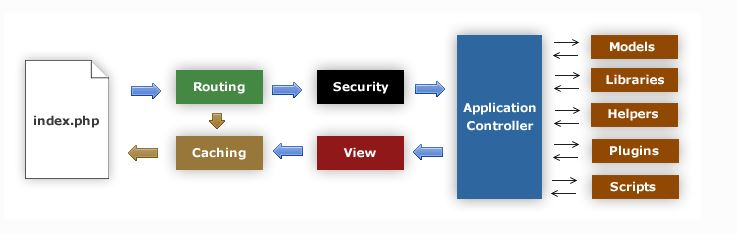
\includegraphics[scale=0.75]{Gambar/flowChartCI}
	\caption{Flowchart CodeIgniter}
	\label{fig:flowchartCI}
\end{figure}

Keterangan:
\begin{enumerate}
	\item Index.php berfungsi sebagai pengontrol utama, yang menginisialisasikan sumber-sumber yang diperlukan untuk menjalankan CodeIgniter.
	\item \textit{Router} akan memeriksa permintaan HTTP untuk menentukan apa yang harus dilakukan selanjutnya
	\item Jika terdapat \textit{cache}, maka cache tersebut akan dikirim langsung ke browser dengan menjalankan sistem eksekusi normal.
	\item  HTTP \textit{request} dan data yang diserahkan oleh \textit{user} akan disaring oleh sistem keamanan terlebih dahulu oleh bagian keamanan(\textit{security}) dari CodeIgniter yang dijalankan sebelum \textit{controller} dari aplikasi diisi.
	\item \textit{Application Controller} akan mengambil isi dari \textit{model, libraries, helpers, plugins, scripts}, dan sumber lain yang diperlukan untuk menjalankan perintah-perintah spesifik.
	\item Kemudian \textit{View} akan diterjemahkan dari \textit{Application Controller} dan dikirim ke \textit{web browser} untuk kemudian ditampilkan. Jika pada view final terdapat \textit{file cache}, maka view tersebut akan terlebih dahulu dilakukan \textit{cached} sehingga permintaan berikutnya dapat dilayani.
\end{enumerate}

\subsection{Model-View-Controller}
\label{sub: MVC}

CodeIgniter menggunakan dasar pola pengembangan \textit{Model-View-Controller}(MVC). Pola pengembangan MVC ini merupakan suatu pendekatan yang memisahkan antara pengerjaan logika dan tampilan dari aplikasi.

MVC sendiri terdiri dari 3 bagian, yaitu:
\begin{enumerate}
	\item \textit{Model} merepresentasikan struktur data. Secara khusus, \textit{model} merupakan kelas yang membantu menangani kueri-kueri sql seperti \textit{insert, update,}dan \textit{delete} pada basis data.
	\item \textit{View} merepresentasikan informasi yang ditunjukkan kepada pengguna. Sebuah \textit{view} biasanya berbentuk \textit{web page}, tetapi dalam CodeIgniter \textit{view} bisa berbentuk \textit{header, footer,} dan berbagai jenis \textit{page} lainnya.
	\item \textit{Controller} berfungsi sebagai perantara antara \textit{Model}, \textit{View}, dan sumber daya lain yang diperlukan untuk memproses HTTP \textit{request} dan menghasilkan halaman web.
\end{enumerate}

\subsection{Controller}
\label{sub: controller}

	\textit{Controller} merupakan sebuah kelas simple dengan penerapan seperti URL. Seperti kelas pada umumnya, ketika nama kelas dari \textit{controller} dan nama kelas dari \textit{file controller} tersebut cocok, maka kelas dapat dijalankan dengan baik. Nama kelas suatu \textit{controller} dikatakan sah jika diawali dengan huruf besar. Untuk lebih jelasnya, perhatikan gambar \ref{fig:controller}.
	
		\begin{figure}[H]
			\centering
			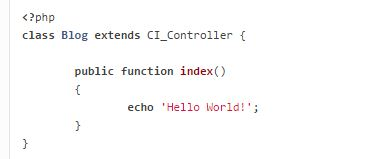
\includegraphics[scale=1]{Gambar/controller}
			\caption{Contoh Kode Controller}
			\label{fig:controller}
		\end{figure}

	Nama \textit{file} pada gambar \ref{fig:controller} haruslah  "Blog.php" dengan B besar dan disimpan pada \textit{application/controllers} sehingga url dapat berjalan dengan baik.
	
\subsubsection{Method}
\label{subsub: method}

	\textit{Method} merupakan nama fungsi dari suatu kelas. Nama \textit{method} pada gambar \ref{fig:controller} adalah \textit{index()}. \textit{Method} bernama "index" akan selalu dijalankan jika tidak ada arahan ke metode pada URL. Cara lain untuk menjalankan \textit{method} pada gambar \ref{fig:controller} adalah "example.com/index.php/blog/index/" dimana bagian terakhir adalah nama method yang ingin dijalankan.
	
	
	\begin{figure}[H]
		\centering
		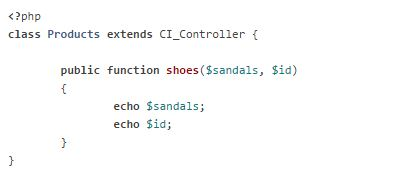
\includegraphics[scale=1]{Gambar/methode}
		\caption{Contoh Method ber-Parameter}
		\label{fig:method}
	\end{figure}
	
	Jika \textit{method} yang dituju memiliki parameter, diperlukan tambahan pada URL pemanggilannya. Sebagai contoh, pemanggilan \textit{method}	pada gambar \ref{fig:method} dilakukan dengan URL "example.com/index.php/products/shoes/sandals/123" dimana "sandals" dan "123" merupakan isi dari \textit{parameter 1} dan 2 dari \textit{method} "shoes".
	
\subsubsection{Mendefinisikan Controller Default}
\label{subsub: defaulController}

	CodeIgniter dapat menjalankan \textit{default controller} sehingga tidak diperlukannya penulisan URL yang lengkap untuk pemanggilan, melainkan \textit{controller} dapat dipanggil secara otomatis dengan URL "example.com" saja. Namun, untuk dapat menjalankan fungsi ini, diperlukan sedikit pengaturan pada \textit{file} "application/config/routes.php" yaitu perubahan variabel pada gambar \ref{fig:route}.
	
	\begin{figure}[H]
		\centering
		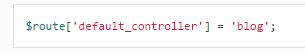
\includegraphics[scale=1]{Gambar/route}
		\caption{Penggantian Variable pada Route}
		\label{fig:route}
	\end{figure}
	
	Pada gambar \ref{fig:route}, "blog" merupakan nama \textit{file} \textit{controller} yang telah dibuat pada direktori "application/controllers/". Setelah pengaturan tersebut, maka pengguna bisa menjalankan aplikasi tanpa URL yang terspesifikasi menjalankan \textit{controller}.
	
	\subsection{Views}
	\label{sub: views}
	
	Sebuah \textit{views} merupakan bagian yang mengatur tampilan aplikasi yang akan ditunjukkan kepada pengguna. \textit{Views} meliputi \textit{footer, header, sidebar,} dll.
	Pada CodeIgniter, \textit{Views} tidak dapat dijalankan secara langsung dari URL, tapi \textit{views} harus dijalankan melalui file \textit{controller} yang ada. Hal ini dilakukan guna memudahkan \textit{programmer} dan mewujudkan \textit{framework MVC} pada CodeIgniter.
	
	\subsubsection{Pembuatan Views}
	\label{subsub: pembuatanView}
	
	Pembuatan \textit{file view} pada dasarnya sama seperti pembuatan \textit{file} berbasis PHP biasa. Gambar \ref{fig:view} merupakan salah satu contoh \textit{file view} sederhana.
	
	\begin{figure}[H]
		\centering
		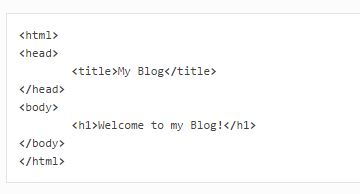
\includegraphics[scale=1]{Gambar/view}
		\caption{Contoh File View}
		\label{fig:view}
	\end{figure}
	
	Setelah selesai membuat \textit{file view} yang diinginkan, maka penyimpanan \textit{file} tersebut harus diletakkan di direktori "application/views/".
	
	\subsubsection{Menjalankan View}
	\label{subsub: menjalankanView}
	
	Menjalankan \textit{view} pada CodeIgniter dilakukan di \textit{file controller}. Gambar \ref{fig:controllerView} menunjukkan kode yang harus ditulis di dalam \textit{method controller}.
	
	\begin{figure}[H]
		\centering
		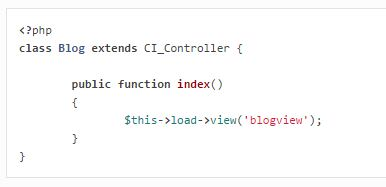
\includegraphics[scale=1]{Gambar/controllerView}
		\caption{Contoh Pemanggilan File View pada Controller}
		\label{fig:controllerView}
	\end{figure}
	
	\subsection{Models}
	\label{sub: models}
	
	\textit{Model} merupakan \textit{file} berbasis PHP yang didesain sebagai penghubung aplikasi dengan basis data. \textit{Model} berfungsi menjalankan kueri-kueri sql seperti \textit{insert, update, delete, select,} dll.
	Pada CodeIgniter terdapat fungsi \textit{Query builder} yang memudahkan \textit{programmer} dalam membuat kueri. Gambar \ref{fig:insert} dan gambar \ref{fig:update} merupakan contoh penggunaan \textit{Query builder} untuk kueri sql \textit{insert} dan \textit{update}.
	
	\begin{figure}[H]
		\centering
		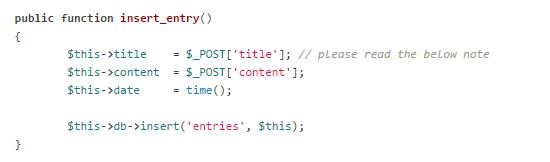
\includegraphics[scale=1]{Gambar/insert}
		\caption{Contoh Query Builder insert}
		\label{fig:insert}
	\end{figure}
	
	\begin{figure}[H]
		\centering
		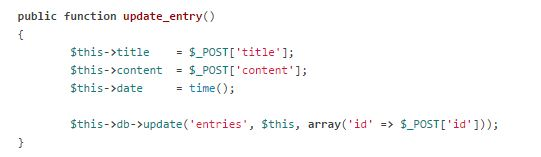
\includegraphics[scale=1]{Gambar/update}
		\caption{Contoh Query Builder Update}
		\label{fig:update}
	\end{figure}
	
	\subsubsection{Menjalankan Model}
	\label{subsub: menjalankanModel}
		
	Sama seperti menjalankan \textit{file view}, \textit{model} pun tidak bisa dijalankan secara langsung menggunakan URL. Untuk menjalankan \textit{model} perlu dilakukan pemanggilan pada \textit{controller}.
	
	\begin{figure}[H]
		\centering
		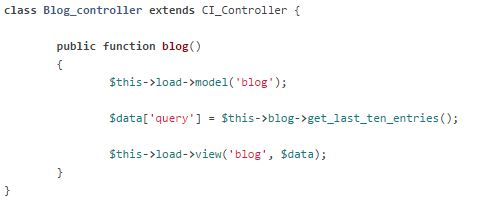
\includegraphics[scale=1]{Gambar/model}
		\caption{Contoh Pemanggilan File Model pada Controller}
		\label{fig:controllermodel}
	\end{figure}
	
	Gambar \ref{fig:controllermodel} menunjukkan bahwa \textit{file controller} melakukan pemanggilan \textit{model} yang diikuti dengan inisialisasi \textit{array data} dari basis data yang dimasukkan ke pemanggilan \textit{view}.
	
	\subsection{Helper}
	\label{sub: helper}
	
	\textit{Helper} merupakan kelas yang membantu \textit{programmer} dalam menjalankan \textit{task}. CodeIgniter memiliki banyak kelas \textit{helper}, seperti \textit{URL Helper} yang membantu dalam membuat \textit{link}, \textit{Form Helper} yang membantu dalam pembuatan elemen-elemen di dalam form, \textit{Text Helper} yang membantu dalam menjalankan berbagai \textit{text formatting routines}, \textit{Cookies Helper} yang membantu dalam mengatur dan membaca \textit{cookies} yang ada, dll. \textit{Helper} pada CodeIgniter umumnya ada pada direktori "application/helpers directory" atau "system/helpers". 
	
	\subsubsection{Menjalankan Helper}
	\label{subsub: menjalnkanHelper}
	
	Cara menjalankan \textit{helper} pada CodeIgniter cukup dengan menambahkan kode pada gambar \ref{fig:kodeHelper} di dalam \textit{kdoeHelper} atau \textit{view}.
	
	\begin{figure}[H]
		\centering
		
\includegraphics[scale=1]{Gambar/helperLoad}
		\caption{Kode yang ditambahkan untuk menjalankan helper}
		\label{fig:kodeHelper}
	\end{figure}
	
	Penulisan "name" pada gambar \ref{fig:kodeHelper} diisi dengan \textit{part helper} yang diinginkan. Contoh jika pada aplikasi perlu \textit{URL Helper} maka "name" diganti dengan "url". Helper juga dapat dijalankan secara otomatis dengan cara mengisi variable 'helper' pada \textit{file autoload} yang berada di direktori "application/config/autoload.php".
	
	\subsection{Basis data}
	\label{sub: database}
	
	\subsubsection{Menyambungkan ke Basis Data}
	\label{subsub: connectDatabase}
	
	Perlu diingat bahwa kelas \textit{model} tidak menjalankan basis data secara otomatis. Untuk membuat aplikasi terkoneksi dengan basis data, diperlukan beberapa tambahan kode pada \textit{file model} atau \textit{file controller}.
	CodeIgniter memiliki fitur \textit{automatically connecting} yang membuat seluruh aplikasi tersambung dengan basis data pada setiap \textit{page load}. untuk mengaktifkan fitur ini cukup mengetikkan "database" pada variabel autoload['libraries'] di "application/config/autoload.php" seperti gambar \ref{fig:autoload}.
	
	\begin{figure}[H]
		\centering
		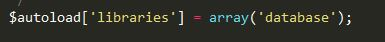
\includegraphics[scale=1]{Gambar/autoload}
		\caption{Kode yang ditambahkan untuk autoload basis data}
		\label{fig:autoload}
	\end{figure}
	
	Selain \textit{autoload}, CodeIgniter juga mendukung koneksi ke basis data dengan cara manual, dengan cara menambahkan "\$this->load->database();" pada \textit{method} atau kelas basis data ingin dijalankan.
	
	\subsection{Konfigurasi Basis Data}
	\label{sub: databaseConf}
	
	Konfigurasi basis data pada CodeIgniter disimpan dengan cara \textit{multi-dimensional array}.
	
	\begin{figure}[H]
		\centering
		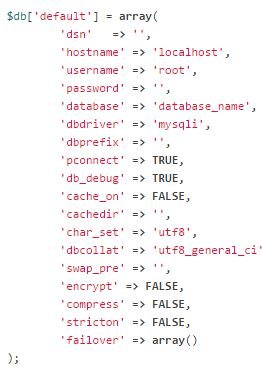
\includegraphics[scale=1]{Gambar/database}
		\caption{Konfigurasi Basis Data}
		\label{fig:database}
	\end{figure}
	
	Keterangan gambar \ref{fig:database}:
	\begin{center}
	\begin{tabular}{| m{5cm} | m{10cm} |}
		\hline
		Nama Konfigurasi & Deskripsi\\
		\hline
		dsn & membuat koneksi string(\textit{an all-in-one configuration sequence})\\
		\hline
		hostname & nama host dari server basis data yang dipakai.(umumnya bernama "localhost")\\
		\hline
		username & username yang dipakai untuk menyambungkan basis data\\
		\hline
		password & password yang cocok dengan username yang dipakai untuk menyambungkan basis data\\
		\hline
		database & nama basis data yang ingin di sambungkan\\
		\hline
		dbdriver & tipe basis data (mysqli, postgre, odbc, dll). Perlu ditulis dengan huruf kecil secara spesifik.\\
		\hline
		dbprefix & dbprefix tidak harus terisi, berguna untuk menambahkan awalan nama tabel pada saat dijalankan Query Builder.\\
		\hline
		pconnect & berisi TRUE atau FALSE untuk perlunya koneksi yang tetap\\
		\hline
		db\_debug & berisi TRUE atau FALSE untuk perlunya menampilkan error dari basis data\\
		\hline
		cache\_on & berisi TRUE atau FALSE untuk diperbolehkannya database query caching\\
		\hline
		cachedir & server path yang mutlak untuk direktori database query cache\\
		\hline
		char\_set & set karakter yang digunakan untuk komunikasi dengan basis data\\
		\hline
		dbcollat & pemeriksaan karakter yang digunakan dalam berkomunikasi dengan basis data(hanya dipakai di driver 'mysqli' dan 'mysql').\\
		\hline
		swap\_pre & sebuah tabel default yang harus bertukar dengan dbprefix.\\
		\hline
		schema & skema basis data yang nilai defaultnya adalah 'public'. Digunakan untuk driver PostgreSQL and ODBC.\\
		\hline
		encrypt &  berisi TRUE atau FALSE perlu tidaknya memakai koneksi yang ter-enkripsi.\\
		\hline
		compress & perlu tidaknya memakai client compression (hanya untuk MYSQl)\\
		\hline
		stricton &  berisi TRUE atau FALSE untuk perlu tidaknya memakai koneksi "Strict Mode" \\
		\hline
		port & nomor port dari basis data. Untuk menggunakannya diperlukan penambahan di config array database.\\
		\hline
	\end{tabular}
\end{center}
	
\section{AngularJS}
\label{sec: angularJS}

AngularJS\cite{AngularJSDocs} merupakan sebuah \textit{framework} terstruktur yang digunakan untuk aplikasi web yang bersifat dinamis. Hal tersebut memungkinkan \textit{programmer} untuk mempergunakan HTML sebagai template bahasa pemrograman dan memperluas sintaks HTML agar dapat mengekspresikan komponen aplikasi dengan jelas dan ringkas. Sifat AngularJS yang mengikat data dan mempunyai ketergantungan injeksi akan menghilangkan banyak kode yang seharusnya dituliskan oleh \textit{programmer}, dan semua itu terjadi pada \textit{browser} sehingga dapat disimpulkan bahwa AngularJS merupakan pasangan yang sangat ideal bagi penggunaan teknologi server. 
Dalam pembuatannya, ketidakcocokkan halaman statik dan dinamik biasanya diselesaikan dengan pendekatan sebagai berikut:
\begin{enumerate}
	\item \textit{Library}: merupakan sebuah koleksi dari berbagai macam fungsi yang berguna dalam pembuatan aplikasi \textit{web}, contoh: JQuery.
	\item \textit{Frameworks}: merupakan suatu implementasi dari sebuah aplikasi \textit{web} yang menempatkan kode yang dituliskan secara detail. \textit{Framework} akan berperan melakukan pemanggilan ke kode yang dituliskan \textit{programmer} ketika aplikasi membutuhkan sesuatu yang spesifik, contoh: durandal, ember, dll.
\end{enumerate}

Dalam pembentukannya, AngularJS memiliki pendekatan yang berbeda. AngularJS berupaya untuk meminimalkan ketidakcocokan antara dokumen utama dari HTML dengan apa yang dibutuhkan oleh aplikasi untuk membuat konstruksi HTML baru. AngularJS mengajarkan \textit{browser} sintaks baru yang disebut \textit{directives}. Contoh contoh \textit{directives} adalah:
\begin{enumerate}
	\item Keterikatan data di dalam \{\{\}\};
	\item Dukungan untuk \textit{Form} dan \textit{Form Validation}
	\item Pengelompokkan HTMl menjadi komponen - komponen yang dapat dipakai kembali.
\end{enumerate}

\subsection{Gambaran Konseptual}
\label{sub: gambaranKonsep}
	Berikut ini adalah beberapa bagian-bagian terpenting dalam AngularJS.
	\begin{center}
		\begin{tabular}{| m{5cm} | m{10cm} |}
			\hline
			Konsep & Deskripsi \\
			\hline
			Template & HTML dengan tambahan markup \\
			\hline
			Directives & Pengembangan HTML dengan atribut dan elemen yang dibuat khusus \\
			\hline
			Model & Data yang ditunjukan kepada pengguna pada tampilan dan bagaimana penguna berinteraksi \\
			\hline
			Scope & Konteks dimana model disimpan, sehingga controller, directives dan expression dapat mengaksesnya \\
			\hline
			Expression & Mengakses variabel dan fungsi dari scope \\
			\hline
			Compiler & Menguraikan template, directives, dan expression \\
			\hline
			Filter & Mengatur nilai dari sebuah expression untuk di tunjukkan kepada pengguna \\
			\hline
			View & Apa yang akan dilihat oleh pengguna (DOM) \\
			\hline
			Data Binding & Menyelaraskan data yang ada pada \textit{model} dan view \\
			\hline
			Controller & Mengatur logika dibalik tampilan \\
			\hline
			Dependency Injection & Membuat dan menyambungkan objek dan fungsi \\
			\hline
			Injector & Tempat penyimpanan dependency Injection \\
			\hline
			Module & Tempat penyimpanan untuk bagian-bagian yang berbeda dalam sebuah aplikasi, yang mencakup: controllers, services, filters, directives yang mengkonfigurasika injector \\
			\hline
			Services & Logika bisnis independen dari views yang bisa dipakai kembali  \\
			\hline
			\end{tabular}
		\end{center}
		
\subsection{Directives}
\label{sub: directives}

	\textit{Directives} merupakan penanda pada \textit{DOM elements} (seperti attribut, nama elemen, \textit{comment},  dan kelas CSS) yang memberitahukan kepada \textit{AngularJS HTML compiler} untuk melampirkan perilaku yang di inginkan kepada \textit{DOM element}(contohnya memakai \textit{event listener}), atau bahkan mengubah \textit{DOM element} yang dituju beserta dengan peranakannya.
	
	AngularJS menyediakan sekumpulan \textit{directives built-in} seperti ng-Model, ng-Bind, dan ng-Class. 
	


\subsection{Data Binding}
\label{sub: dataBinding}
	
	\textit{Data Binding} pada AngularJS merupakan penyelarasan data antara \textit{model} dan komponen - komponen \textit{view}. Ketika \textit{model} berubah, maka \textit{view} pun akan berubah, begitu juga dengan sebaliknya.
	
	\begin{figure}[H]
		\centering
		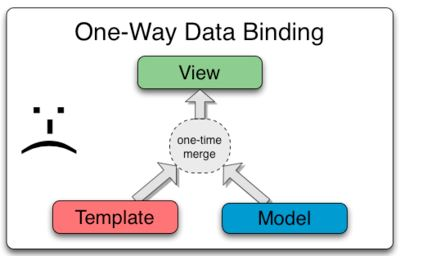
\includegraphics[scale=0.75]{Gambar/Dabin1}
		\caption{Data Binding Classical Templates System}
		\label{fig:dabin1}
	\end{figure}
	Pada gambar \ref{fig:dabin1} menjelaskan bahwa kebanyakan \textit{data binding} adalah proses satu arah. Hal itu dilakukan dengan menyatukan \textit{template} dan \textit{model} menjadi \textit{view}. Setelah penyatuan, pergantian pada \textit{model} tidak secara otomatis mengganti \textit{view} yang sudah ditampilkan.
	\begin{figure}[H]
		\centering
		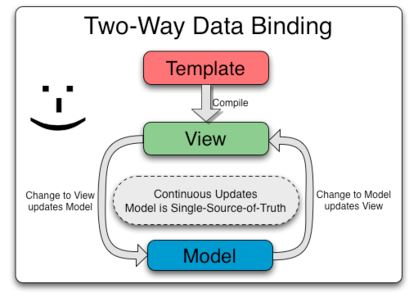
\includegraphics[scale=0.75]{Gambar/Dabin2}
		\caption{Data Binding pada Angular}
		\label{fig:dabin2}
	\end{figure}
	Pada gambar \ref{fig:dabin2} menjelaskan perbedaan yang diberikan oleh pelaksanaan \textit{data binding} pada AngularJS. Pertama, \textit{template} akan di \textit{compile} pada browser. Hasil dari \textit{compile} tersebut adalah \textit{live view}. Pada tahap ini perubahan yang terjadi di \textit{view} akan disampaikan kepada \textit{model}, dan perubahan yang terjadi pada \textit{model} akan mengubah \textit{view}.
	
	Karena \textit{view} merupakan proyeksi dari \textit{model}, menyebabkan \textit{controller} benar-benar terpisahkan dari \textit{view} tanpa disadari. Hal ini mempermudah pengujian \textit{controller}, karena terisolasi tanpa adanya \textit{view} dan DOM( \textit{browser dependency}).
	
\subsection{Model-View-Controller(MVC)}
\label{sub: mvcAngular}

	AngularJS\cite{green2013angularjs} juga merupakan salah satu \textit{framework} yang menggunakan  \textit{Model-View-Controller} sebagai patokan desain aplikasi. Walaupun AngularJS mempunyai banyak flexibilitas dalam membangun aplikasi, tetapi akan ada beberapa hal yang selalu dijumpai dalam mendesain sbuah aplikasi, diantaranya:
	\begin{itemize}
		\item Sebuah \textit{model} selalu menampung data yang merepresentasikan keadaan aplikasi.
		\item \textit{Views} yang menyajikan data tersebut.
		\item \textit{Controller} yang akan selalu mengatur hubungan antara \textit{model} dan \textit{views}.
	\end{itemize}
	
	Model dibuat dengan menggunakan atribut berupa objek atau konten-konten primitif yang dapat menyimpan data. Berikut adalah salah satu contoh praktis dalam pembuatan \textit{model}:
\begin{lstlisting}
var someText = 'You have started your journey.'
\end{lstlisting}
	Setelah itu untuk menampilkannya maka perlu dibuat \textit{view} dari data \textit{model} "someText" diatas dengan cara:
\begin{lstlisting}
<p> {{someText}} </p>
\end{lstlisting}
	\textit{Syntax view} 2 kurung kurawal diatas disebut sebagai interlopasi(penyusupan), karena hal tersebut memasukkan konten baru ke dalam \textit{template} yang sudah ada.\\
	Sementara kelas \textit{controllers} berguna untuk memberitahu AngularJS tentang objek atau konten primitif mana dari model yang akan dipakai dengan cara menetapkannya ke objek '\$scope ', objek '\$scope' tersebut kemudian akan diberikan kepada \textit{controller} seperti contoh berikut:
\begin{lstlisting}
function TextController($scope){
	$scope.someText = someText;
}
\end{lstlisting}
	
	Berikut ini adalah contoh penggabungan fungsi \textit{model, view,} dan \textit{controller}:
\begin{lstlisting}
<html>
<body ng-controller = "TextController">
	<p>{{someText}}</p>
	
	<script>
		src="https://ajax.googleapis.com/ajax/libs/angularjs/1.0.4/angular.min.js">
	</script>
	
	<script>
		function TextController($scope){
			$scope.someText = 'You have started your journey.';
		}
	</script>
</body>
</html>
\end{lstlisting}
	
	Hasil dari kode diatas adalah tulisan "You have started your journey". Walaupun cara ini dapat dilakukan dengan mudah pada aplikasi sederhana seperti contoh diatas, tetapi untuk kebanyakan aplikasi sebaiknya dibuat objek model untuk menyimpan \textit{data} yang ada. Untuk itu, daripada membuat model seperti:
	
\begin{lstlisting}
function TextController($scope){
	$scope.someText = someText;
}
\end{lstlisting}
	
	Lebih baik menggunakan kode:
\begin{lstlisting}
var message= {};
message.someText = 'You have started your journey';
function TextController($scope){
	$scope.message = message;
}
\end{lstlisting}
	Yang kemudian akan dipanggil di \textit{template} dengan kode:
\begin{lstlisting}
<p>{{message.someText}}</p>
\end{lstlisting}
	Perubahan yang dilakukan diatas berfungsi untuk mencegah perilaku tidak terduga yang dapat terjadi dari \textit{prototypal inheritance} dalam objek \$scope. Walaupun untuk sementara hal ini dapat berjalan dengan baik, tetapi cara yang benar dalam mendefinisikan sebuah \textit{controller} adalah dengan menggunakan sebuah kelas yang dinamakan \textit{module} yang menyediakan \textit{namespace} untuk bagian lain dari aplikasi berhubungan. Perubahan tersebut akan mengubah kode-kode diatas menjadi:
	\begin{lstlisting}
<html ng-app='myApp'>
<body ng-controller='TextController'>
	<p>{{someText.message}}</p>
	<script>
		src="https://ajax.googleapis.com/ajax/libs/angularjs/1.0.4/angular.min.js">
	</script>
	
	<script>
		var myAppModule = angular.module('myApp',[]);
		
		myAppModule.controller('TextController',
			function($scope){
			var someText = {};
			someText.message = 'You have started your journey';
			$scope.someText = someText;
		});
	</script>
</body>
</html>
	\end{lstlisting}
	Pada versi di atas, aplikasi memberi tahu elemen ng-app tentang nama dari modul yang dipakai di baris ke 9. Setelah itu pada baris ke 11 sampai 16 dilakukan pemanggilan objek Angular untuk membuat sebuah modul bernama myApp dan memberikan fungsi dari \textit{controller} untuk memanggil fungsi controller dari modul.
	
\section{Twitter Bootstrap}
\label{sec: Bootrstrap}

\textit{Twitter Bootstrap}\cite{bootstrap} atau yang lebih dikenal dengan \textit{Bootstrap} adalah \textit{framework} HTML, CSS, dan JS terpopuler dalam hal pengembangan tampilan yang responsif \textit{mobile} pertama dalam hal aplikasi berbasis web. 

\subsection{Grid System}
\label{sub: gridSystem}

\textit{Bootstrap} merupakan responsif \textit{mobile} pertama yang mempunyai sistem skala (\textit{grid system}). Sistem skala tersebut membagi layar perangkat menjadi 12 kolom yang berukuran sama, dimana besar ukuran masing-masing kolom mengikuti besar layar perangkat. Ketika layar semakin besar, maka ukuran masing-masing kolom pun akan semakin besar, begitu juga sebaliknya. Cara sistem skala \textit{Bootstrap} bekerja adalah:

\begin{enumerate}
	\item \textit{Rows} harus ditempatkan diantara \textit{.container(fixed-width)} atau \textit{.container-fluid (full-width)} untuk mendapatkan keselarasan ukuran
	\item \textit{Rows} dipergunakan untuk membuat grup kolom secara \textit{horizontal}.
	\item Konten tampilan harus berada diantara kelas \textit{columns} atau peranakan dari kelas \textit{columns}.
	\item Kelas-kelas yang telah ditetapkan seperti ".row" dan ".col-xs-4" dapat digunakan dengan segera untuk membentuk \textit{layout}.
	\item Kelas \textit{columns} membuat \textit{gutters}(jarak antara kolum konten) menggunakan kelas \textit{padding}.
	\item \textit{Grid columns} dibuat dengan menyesuaikan ke-12 kolom yang sudah disediakan. Contohnya jika ingin membuat 3 kolom sama rata, maka diperlukan 3 buah kelas ".col-xs-4".
	\item Jika ada lebih dari 12 kolom dalam 1 baris, maka kolom yang lebih tersebut akan dipindahkan ke baris baru sebagai satu kesatuan.
	\item Kelas \textit{grid} mempunyai fungsi untuk menyesuaikan ukuran sesuai dengan patokan ukuran yang sudah diberikan oleh \textit{bootstrap} atau lebih besar dari angka patokan yang ada. Oleh karena itu ketika sebuah kelas ".col-md-*" tidak memiliki kelas yang lebih besar darinya seperti kelas ".col-lg-*", maka kelas md akan mengambil alih pada saat aplikasi dijalankan di ukuran perangkat yang lebih besar. 
\end{enumerate}
	
\begin{figure}[H]
	\centering
	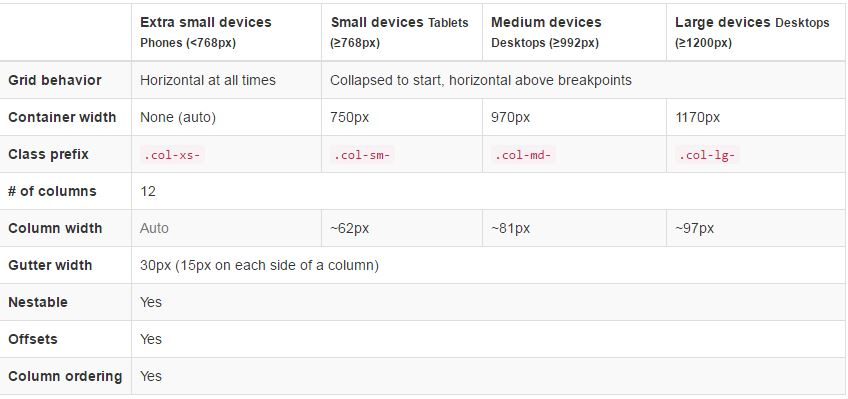
\includegraphics[scale=0.75]{Gambar/gridOption}
	\caption{Grid Option pada Bootstrap}
	\label{fig:gridOpt}
\end{figure}

\begin{figure}[H]
	\centering
	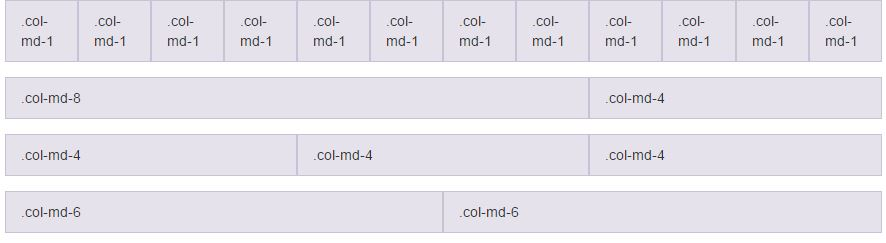
\includegraphics[scale=0.75]{Gambar/kolom}
	\caption{Contoh Pembagian Grid Columns}
	\label{fig:gridCol}
\end{figure}

\subsection{Form Class}
\label{sub: formClass}
	Masing-masing form akan memiliki bentuk otomatis yang diatur secara global. Dengan memakai kelas ".form-control", pengaturan ukuran dari kelas <input>, <textarea>, dan <select> akan otomatis memiliki variabel \textit{width} 100\% secara \textit{default}. Untuk mendapatkan jarak \textit{spacing} yang maksimal, \textit{Bootstrap} memiliki kelas ".form-group" yang membungkus kelas \textit{form} menjadi grup-grup.
	
\begin{figure}[H]
	\centering
	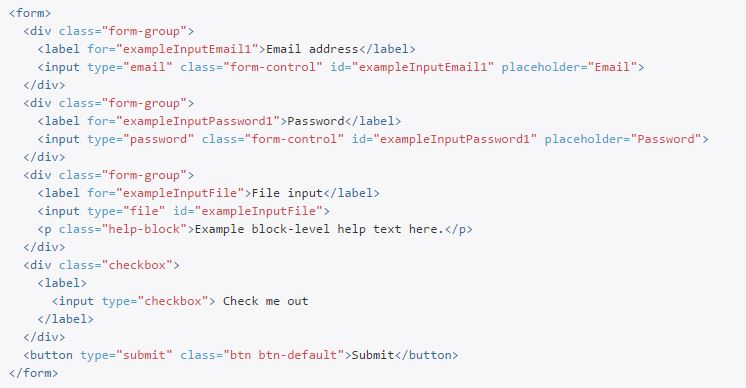
\includegraphics[scale=0.75]{Gambar/formCode}
	\caption{Contoh Penggunaan Kelas Form}
	\label{fig:formCode}
\end{figure}

\begin{figure}[H]
	\centering
	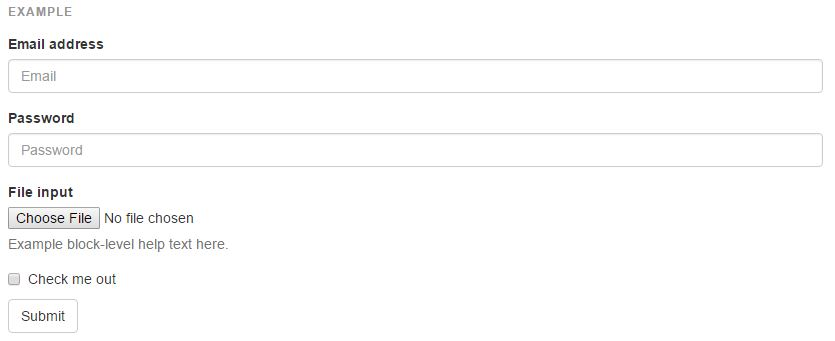
\includegraphics[scale=0.75]{Gambar/hasilForm}
	\caption{Contoh Hasil Pengggunaan Kelas Form}
	\label{fig:hasilForm}
\end{figure}}{}
\ifdefstring{\vbabc}{1}{\chapter{Analisis}
\label{chap: analisis}

\section{Analisis Data Penilaian Skripsi}
\label{sec: analisisData}

	Berdasarkan analisa dari contoh form penilaian skripsi yang ada, dapat disimpulkan bahwa penilaian skripsi membutuhkan data-data sebagai berikut:
		
		\begin{enumerate}
			\item Semester
			\item Tahun ajaran
			\item NPM mahasiswa 
			\item Nama mahasiswa
			\item Judul skripsi
			\item Nama pembimbing utama/tunggal
			\item Nama pembimbing pendamping(tidak harus)
			\item Nama ketua tim penguji
			\item Nama anggota tim penguji
			\item Bobot ketua tim penguji
			\item Bobot anggota tim penguji
			\item Bobot pembimbing
			\item Nilai koordinator skripsi
			\item Bobot koordinator skripsi
			\item Bobot tata tulis laporan ketua
			\item Bobot kelengkapan materi ketua
			\item Bobot penguasaan materi ketua
			\item Bobot presentasi ketua
			\item Bobot pencapaian tujuan ketua
			\item Bobot tata tulis laporan anggota
			\item Bobot kelengkapan materi anggota
			\item Bobot penguasaan materi anggota
			\item Bobot presentasi anggota
			\item Bobot pencapaian tujuan anggota
			\item Bobot tata tulis laporan pembimbing
			\item Bobot kelengkapan materi pembimbing
			\item Bobot penguasaan materi pembimbing
			\item Bobot bimbingan pembimbing
			\item Nilai akhir mahasiswa
		\end{enumerate}
	
	Berdasarkan diskusi dengan dosen pembimbing, disimpulkan bahwa sistem penilaian sidang skripsi 2 ini hanya memerlukan penyimpanan untuk bobot masing-masing penilaian dan nilai akhir mahasiswa untuk tahap perhitungan. Hal ini dikarenakan nilai-nilai lainnya dapat dihasilkan dengan melakukan perhitungan pada  nilai akhir mahasiswa dan bobot nilai yang diinginkan. Begitu pula dengan nilai dari masing-masing penguji.
	
		\begin{figure}[H]
			\centering
			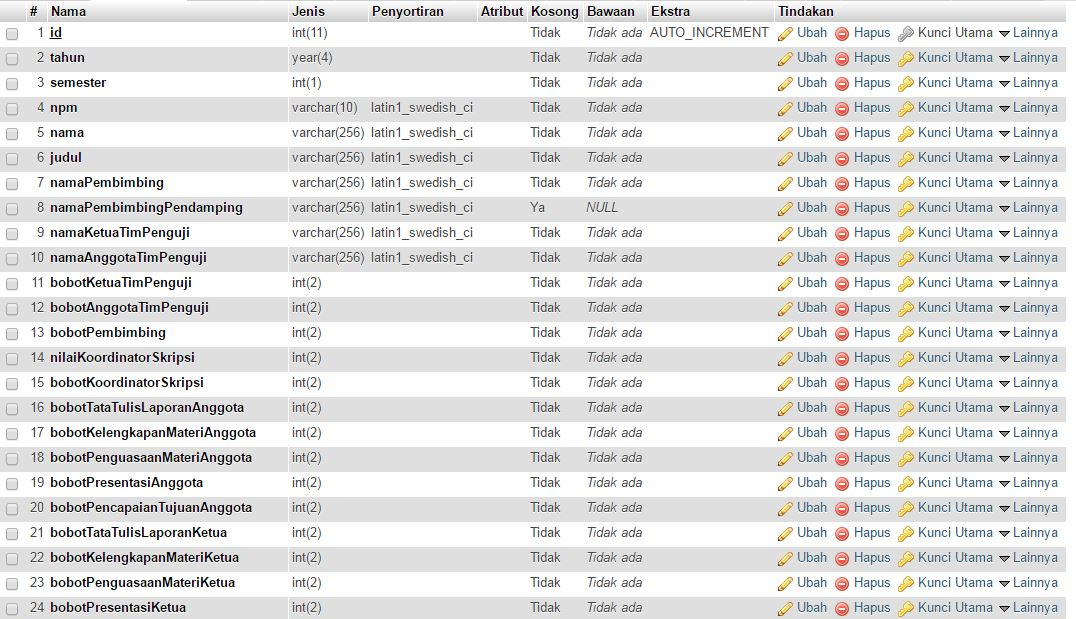
\includegraphics[scale= 1.0]{Gambar/database1}
			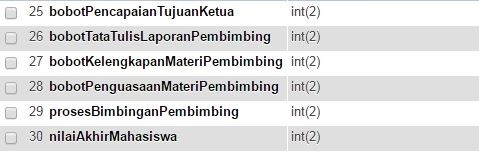
\includegraphics[scale= 1.0]{Gambar/database2}
			\caption {Data yang disimpan di database}
			\label{fig:tabeldata}
		\end{figure}
	
\section{Analisis Tampilan Sistem Informasi Penilaian Skripsi}
\label{sec: analisisTampilan}
	
	Tampilan pada sistem informasi penilaian skripsi haruslah dibuat semirip mungkin dengan form penilaian skripsi yang sudah ada seperti pada lampiran gambar \ref{fig: skripsiAsli} dan gambar \ref{fig: rekapAsli}.
	
	Perbedaan yang akan ditampilkan adalah dengan adanya otomatisasi penghitungan nilai sesuai dengan bobot yang diberikan kepada penilai. Hal ini akan memberikan kemudahan penilai untuk melakukan penilaian.
	
	Gambar \ref{fig:tampilan} adalah bayangan awal tampilan untuk sistem informasi penilaian skripsi:
	\begin{figure}[H]
		\centering
		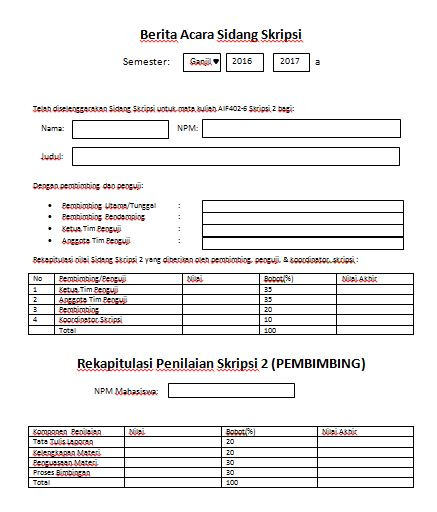
\includegraphics[scale=0.75]{Gambar/tampilan1}
		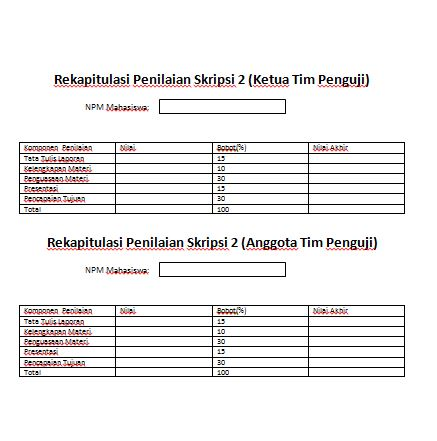
\includegraphics[scale=0.75]{Gambar/tampilan2}
		\caption{Perkiraan Tampilan}
		\label{fig:tampilan}
	\end{figure}
	
	Dari bayangan awal itulah, saya mendesain tampilan dari aplikasi sistem informasi penilaian skripsi 2 ini. Gambar \ref{fig:tampilanapp} merupakan tampilan pada aplikasi sistem informasi penilaian skripsi 2.
	
	\begin{figure}[H]
		\centering
		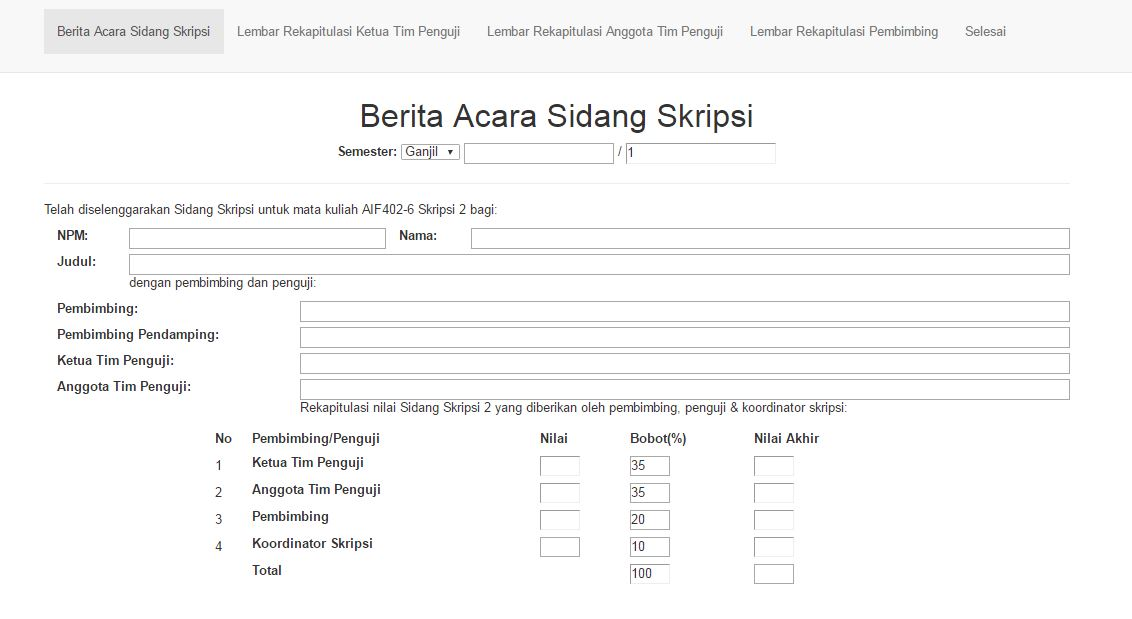
\includegraphics[scale=0.5]{Gambar/tampilanapp1}
		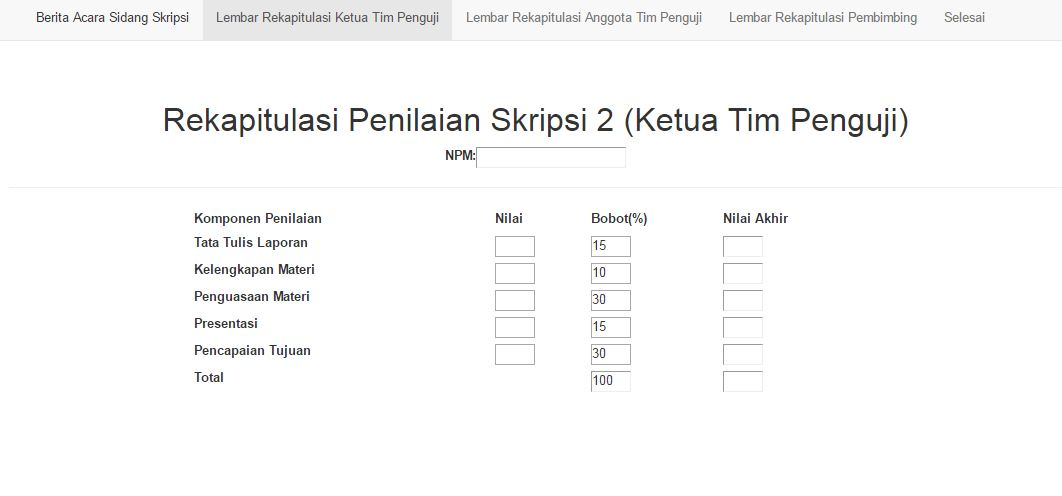
\includegraphics[scale=0.5]{Gambar/tampilanapp2}
		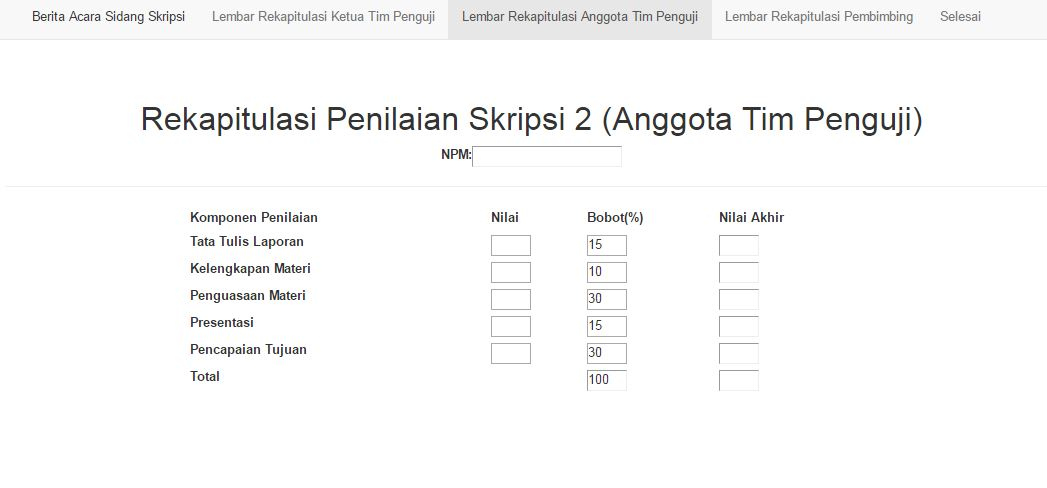
\includegraphics[scale=0.5]{Gambar/tampilanapp3}
		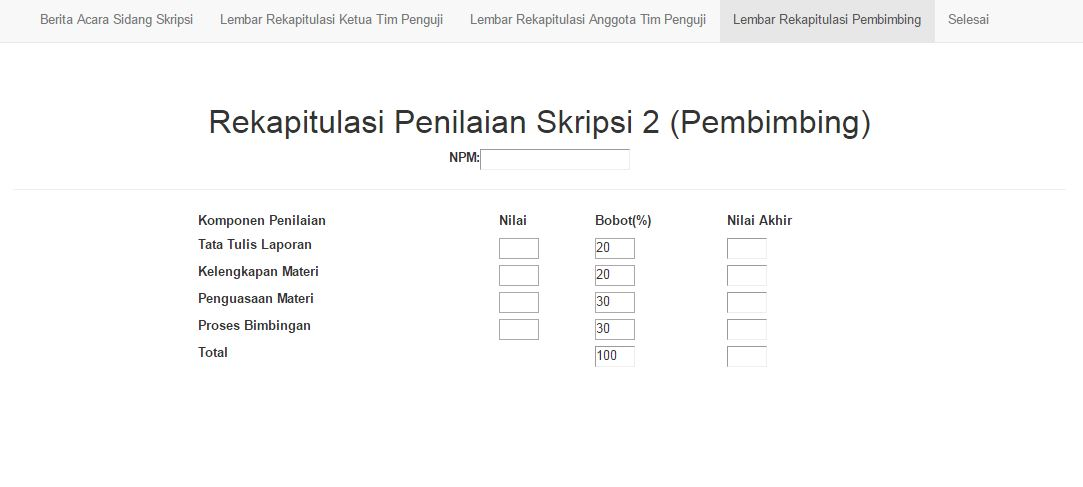
\includegraphics[scale=0.5]{Gambar/tampilanapp4}
		\caption{Perkiraan Tampilan}
		\label{fig:tampilanapp}
	\end{figure}}{}
\ifdefstring{\vbabd}{1}{\chapter{Perancangan}
\label{chap: perancangan}
	
	Pada bab ini akan dijelaskan mengenai perancangan aplikasi yang dibangun meliputi perancangan kelas, \textit{routes}, \textit{controllers}, \textit{models}, perancangan antarmuka.
	
	\section{Perancangan Kelas}
	\label{sec: rancangKelas}
	
	Seperti yang sudah di jelaskan pada bab sebelumnya, untuk memodelkan sistem penilaian sidang skripsi 2 dengan menggunakan \textit{codeigniter} membutuhkan \textit{routes}, \textit{controllers}, \textit{models}, dan \textit{views}. Hal-hal berikut akan dijelaskan pada subbab selanjutnya.
	
	\section{Routes}
	\label{sec: routes}
	
	\textit{Routes} merupakan bagian dari \textit{codeigniter} untuk melakukan pemetaan terhadap lokasi \textit{file controllers} dari aplikasi. Berikut adalah isi dari "config/routes":
	\begin{lstlisting}
		$route['default_controller'] = 'C_skripsi';
		$route['404_override] ="";
		$route[translate_url_dahses'] =	FALSE;
	\end{lstlisting}
	Baris pertama dari kode di atas adalah nama \textit{file controller} yang terletak di \textit{folder controllers} yang akan diambil. Baris kedua merupakan kode untuk menangani \textit{error} yang terjadi jika \textit{file} yang dicari tidak ditemukan, contoh penggunaanya adalah "\$route['404\_override'] = 'errors/page\_missing;". Baris ketiga mempunyai fungsi mengganti seluruh nama \textit{file} yang mengandung '-' menjadi '\_', contoh penggunaanya adalah: "my-controller/index"	menjadi "my\_controller/index".

	\section{Controllers}
	\label{sec: controllers}
	
	\textit{Controller} terdiri dari sebuah kelas yang dinamakan "C\_Skripsi". Keseluruhan aktivitas dari sistem informasi penilaian skripsi diatur oleh kelas ini. Berikut adalah gambar kelas diagram dari \textit{controllers}:
	\begin{figure}[H]
		\centering
		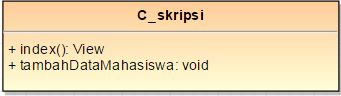
\includegraphics[scale= 1.0]{Gambar/C_skripsi}
		\caption {Gambar diagram kelas \textit{file controllers}}
		\label{fig:controllers}
	\end{figure}
	
	\begin{itemize}
		\item public function index()\\
		Berfungsi untuk mengarahkan pengguna ke \textit{file views default} dari aplikasi.
		\item public function tambahDataMahasiswa()\\
		Berfungsi untuk mengambil data dari \textit{view} yang tersedia, untuk kemudian diolah menjadi bahasa sql oleh \textit{models}.
	\end{itemize}
	
	\section{Models}
	\label{sec: models}
	
	\textit{Models} mempunyai fungsi menghubungkan \textit{views} dan \textit{controllers} pada basis data. Pada penggunaan \textit{codeigniter}, \textit{model} dibuat dengan sangat sederhana. Berikut adalah isi dari kelas model:
	\begin{lstlisting}
		<?php
			defined('BASEPATH') OR exit('No direct script access allowed');
			
			class Skripsi_model extends CI_Model {
			
			public function insertDataMahasiswa($tableName, $data){
				$res = $this->db->insert($tableName, $data);
			}
		}
		
	\end{lstlisting}
	
	\begin{itemize}
		\item public function insertDataMahasiswa(\$tablename, \$data)\\
		Berfungsi untuk mengolah data yang sudah diolah oleh \textit{controllers} menjadi kueri sql \textit{insert data}.
	\end{itemize}
	
	\section{Perancangan Basis Data}
	\label{sec: perancanganDatabase}
	
	Berdasarkan analisis basis data pada bab \ref{sub: analisisDatabase}, maka dibuat tabel basis data.
	\begin{table}[H]
	\centering
	\caption{Tabel Perancangan Basis Data}
	\begin{tabular}{| m{0.75cm} | m{7cm} | m{3cm} |}
		\hline
		No & Nama Tabel & Jenis Data\\
		\hline
		1 & \underline{id} & int(11)\\
		\hline
		2 & tahun & year(4)\\
		\hline
		3 & semester & int(1)\\
		\hline
		4 & npm & varchar(10)\\
		\hline
		5 & nama & varchar(256)\\
		\hline
		6 & judul & varchar(256)\\
		\hline
		7 & namaPembimbing & varchar(256)\\
		\hline
		8 & namaPembimbingPendamping & varchar(256)\\
		\hline
		9 & namaKetuaTimPenguji & varchar(256)\\
		\hline
		10 & namaAnggotaTimPenguji & varchar(256)\\
		\hline
		11 & bobotKetuaTimPenguji & int(2)\\
		\hline
		12 & bobotAnggotaTimPenguji & int(2)\\
		\hline
		13 & bobotPembimbing & int(2)\\
		\hline
		14 & nilaiKoordinatorSkripsi & int(2)\\
		\hline
		15 & bobotKoordinatorSkripsi & int(2)\\
		\hline
		16 & bobotTataTulisLaporanAnggota & int(2)\\
		\hline
		17 & bobotKelengkapanMateriAnggota & int(2)\\
		\hline
		18 & bobotPenguasaanMateriAnggota & int(2)\\
		\hline
		19 & bobotPresentasiAnggota & int(2)\\
		\hline
		20 & bobotPencapaianTujuanAnggota & int(2)\\
		\hline
		21 & bobotTataTulisLaporanKetua & int(2)\\
		\hline
		22 & bobotKelengkapanMateriKetua & int(2)\\
		\hline
		23 & bobotPenguasaanMateriKetua & int(2)\\
		\hline
		24 & bobotPresentasiKetua & int(2)\\
		\hline
		25 & bobotPencapaianTujuanKetua & int(2)\\
		\hline
		26 & bobotTataTulisLaporanPembimbing & int(2)\\
		\hline
		27 & bobotKelengkapanMateriPembimbing & int(2)\\
		\hline
		28 & bobotPenguasaanMateriPembimbing & int(2)\\
		\hline
		29 & prosesBimbinganPembimbing & int(2)\\
		\hline
		30 & nilaiAkhirMahasiswa & int(2)\\
		\hline
		\end{tabular}
	\end{table}
	
	\section{Perancangan Tampilan}
	\label{sec: perancanganTampilan}
	
	Tampilan pada sistem informasi penilaian skripsi haruslah dibuat semirip mungkin dengan form penilaian skripsi yang sudah ada seperti pada lampiran gambar \ref{fig: skripsiAsli} dan gambar \ref{fig: rekapAsli}.
	
	Perbedaan yang akan ditampilkan adalah dengan adanya otomatisasi penghitungan nilai sesuai dengan bobot yang diberikan kepada penilai. Hal ini akan memberikan kemudahan penilai untuk melakukan penilaian.
	
	Gambar \ref{fig:tampilan} adalah bayangan awal tampilan untuk sistem informasi penilaian skripsi:
	\begin{figure}[H]
		\centering
		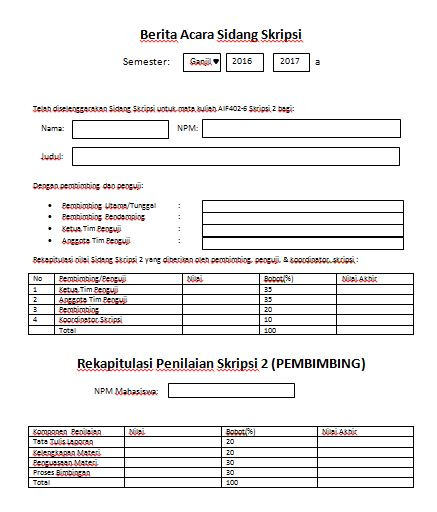
\includegraphics[scale=0.75]{Gambar/tampilan1}
		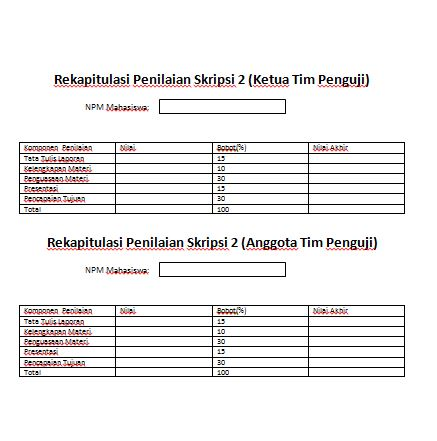
\includegraphics[scale=0.75]{Gambar/tampilan2}
		\caption{Perkiraan Tampilan}
		\label{fig:tampilan}
	\end{figure}}{}
\ifdefstring{\vbabe}{1}{\chapter{Implementasi dan Pengujian}
\label{chap: implemenPengujian}

Pada bagian ini merupakan rincian atau penjelasan lanjut mengenai lingkungan implementasi perangkat keras maupun perangkat lunak sistem informasi penilaian sidang skripsi 2. Bagian terakhir akan membahas tentang pengujian yang telah dilakukan pada sistem informasi.

\section{Implementasi}
\label{sec: implementasi}

	Pada bagian ini akan dijabarkan lingkungan pengembangan sistem informasi dan pengujian.
	
	\subsection{Lingkungan Implementasi dan Pengujian}
	\label{sub: lingkunganImp}
	
	Impelementasi dilakukan dengan menggunakan sebuah laptop. Berikut adalah spesifikasi laptop
	yang digunakan:
	
	\begin{enumerate}
		\item Processor: Intel(R) Core(TM) i5-3230M CPU @ 2.60GHz (4CPUs),~2.6GHz
		\item RAM : 4096 MB
		\item Sistem operasi : Windows 7 Ultimate 64-bit (6.1, Build 7601)
		\item Versi AngularJS : Version 1.5.2
		\item Versi Codeigniter : Version 3.1.3
		\item Versi TwitterBootstrap : Version 2.3.2
		\item Versi Google Chrome : Version 55.0.2883.87 m(64-bit)
	\end{enumerate}

	\subsection{Hasil Implementasi}
	\label{sub: hasilImplemen}
	
	Hasil implementasi dari penelitian ini adalah sebuah sistem informasi berbasis web yang menggunakan \textit{codeigniter}, \textit{AngularJS}, dan \textit{Twitter Bootstrap} sebagai dasar pembuatan. Aplikasi dapat diakses melalui jaringan \textit{global} dengan URL " http://sipskripsi.com ". Sistem informasi terdiri dari bagian-bagian sebagai berikut:
	
	\begin{enumerate}
		\item Bagian formulir berita acara sidang skripsi\\
		Bagian ini adalah halaman yang bersangkutan dalam pengisian data diri mahasiswa yang bersangkutan, sekaligus sebagai halaman akhir yang menyimpulkan perhitungan nilai akhir mahasiswa. Kolom penilaian pada halaman ini tidak dapat diisi secara manual kecuali kolom penilaian milik koordinator skripsi. Kolom penilaian yang lain didapatkan berdasarkan perhitungan nilai akhir masing-masing penguji.
		\begin{figure}[H]
			\centering
			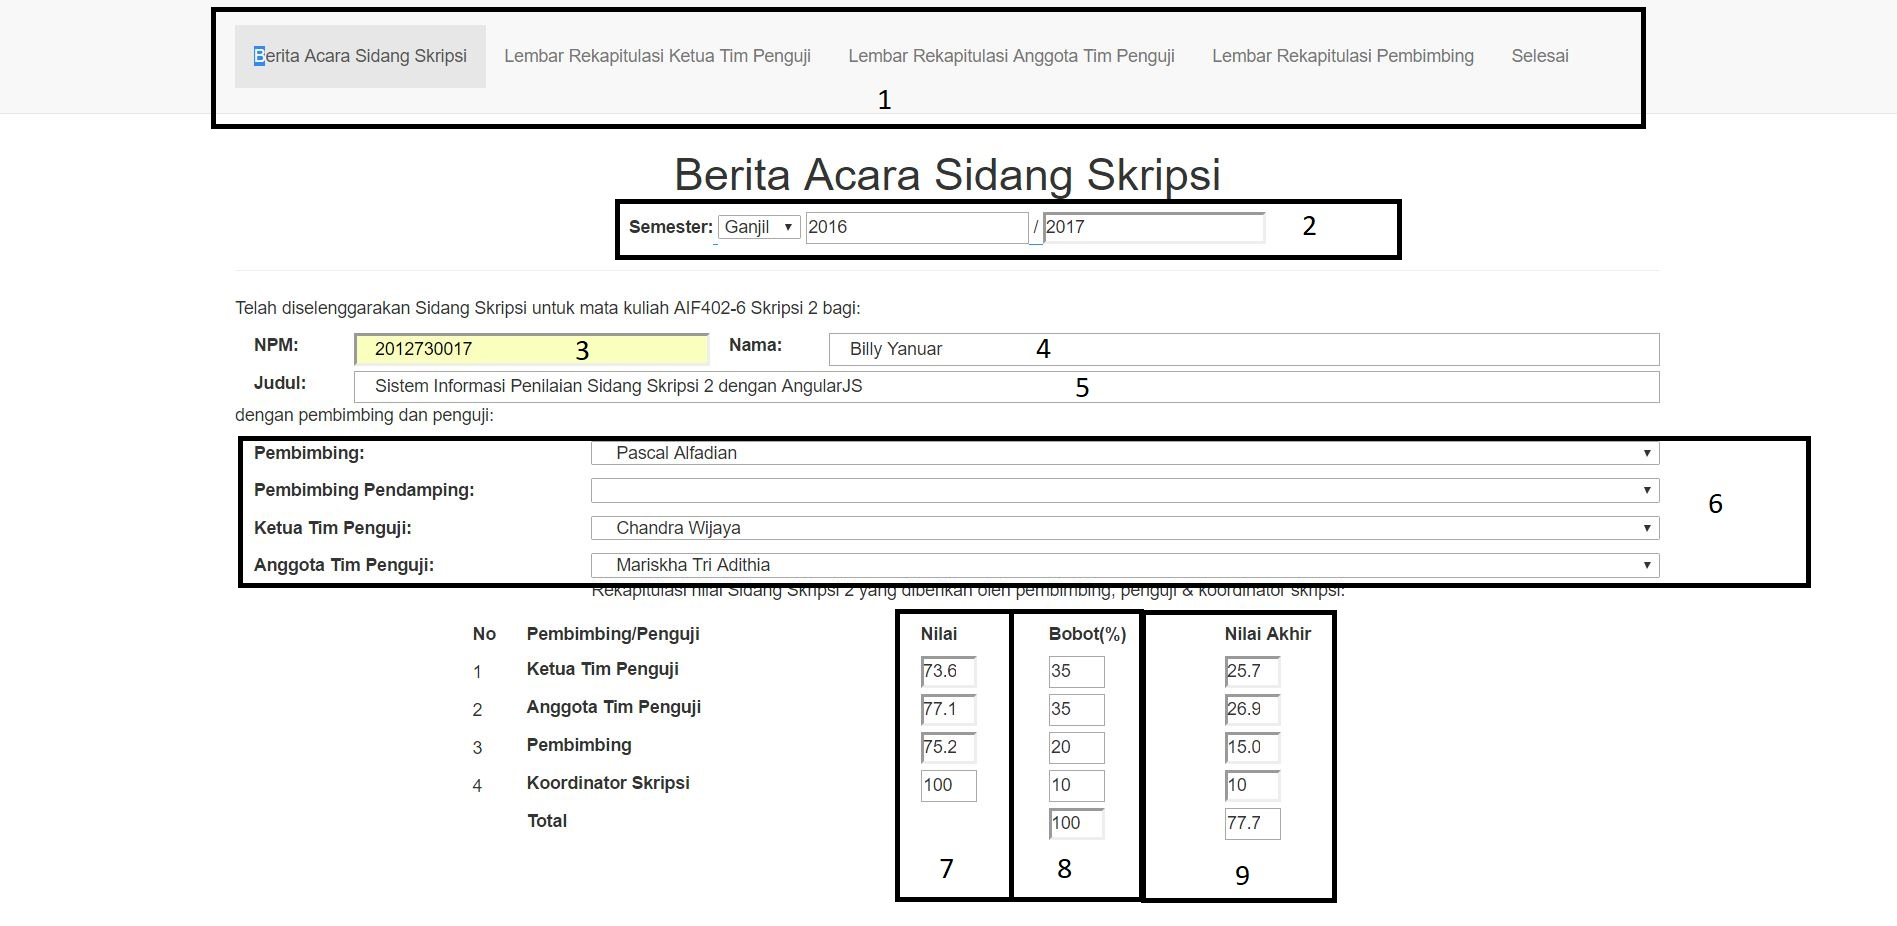
\includegraphics[scale=0.5]{Gambar/beritaacaraisi}
			\caption{Formulir berita acara sidang skripsi 2 terisi}
			\label{fig:beritaisi}
		\end{figure}
		\item Bagian formulir rekapitulasi penilaian sidang skripsi 2.\\
		Bagian ini adalah halaman yang bersangkutan dalam menampung nilai-nilai yang diberikan oleh ketua tim penguji, anggota tim penguji, dan pembimbing pada mahasiswa. 
		\begin{figure}[H]
			\centering
			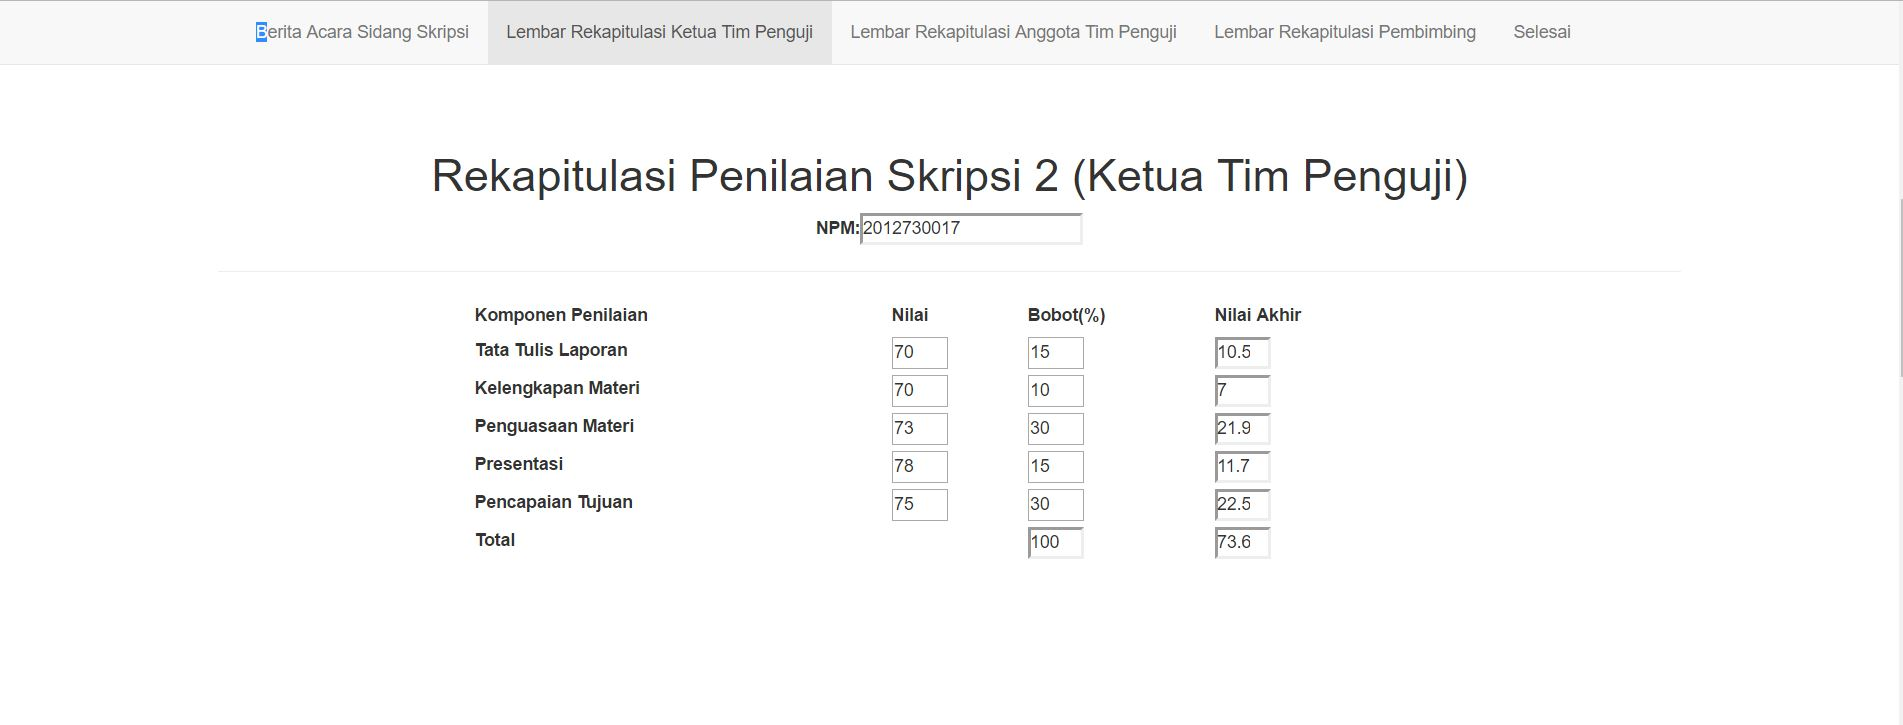
\includegraphics[scale=0.5]{Gambar/ketuaisi}
			\caption{Formulir rekapitulasi ketua tim penguji terisi}
			\label{fig:ketuaisi}
		\end{figure}
		\begin{figure}[H]
			\centering
			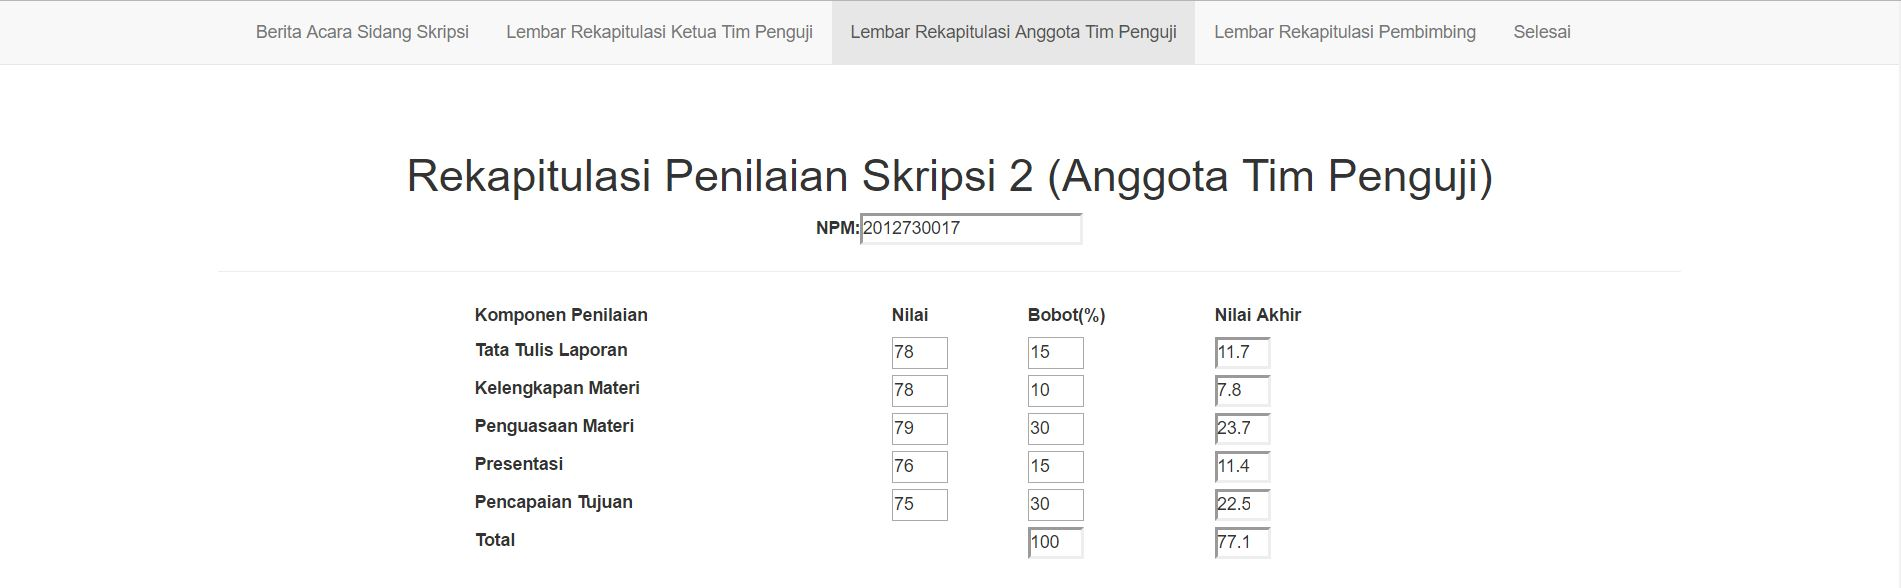
\includegraphics[scale=0.5]{Gambar/anggotaisi}
			\caption{Formulir rekapitulasi anggota tim penguji terisi}
			\label{fig:anggotaisi}
		\end{figure}
		\begin{figure}[H]
			\centering
			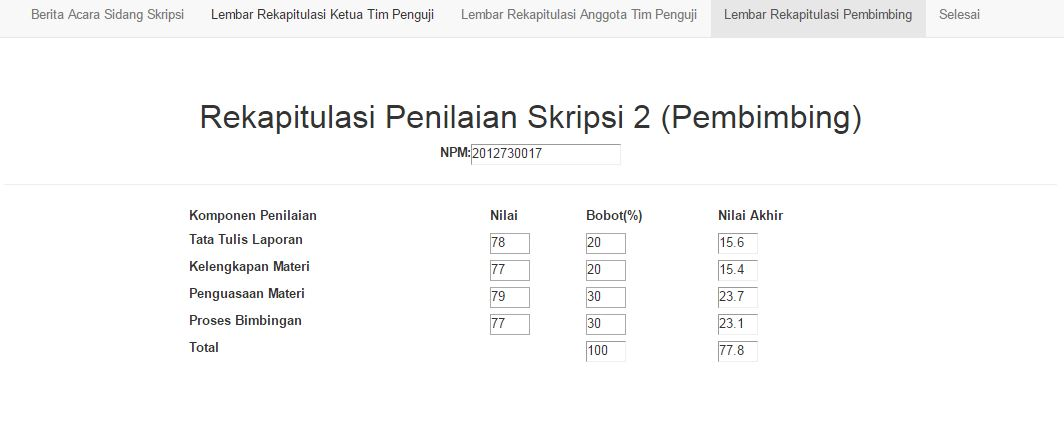
\includegraphics[scale=0.5]{Gambar/pembimbingisi}
			\caption{Formulir rekapitulasi pembimbing terisi}
			\label{fig:pembimbingisi}
		\end{figure}
		\item Bagian selesai.\\
		Bagian ini adalah bagian terakhir dari sistem informasi. Ketika formulir sudah selesai diisi, maka dengan menekan tombol selesai pada bagian ini, \textit{data} yang telah terisi akan dimasukkan ke dalam \textit{database}.
		\begin{figure}[H]
			\centering
			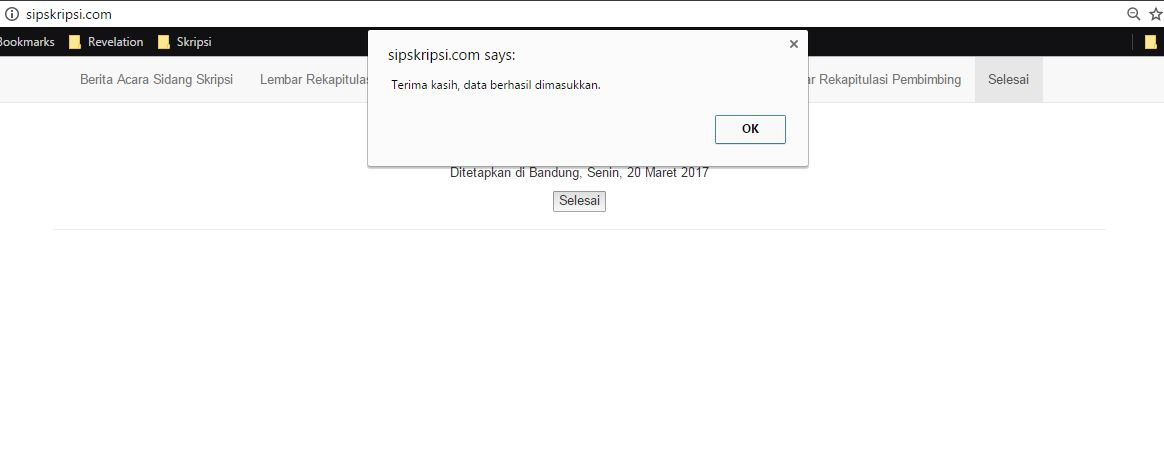
\includegraphics[scale=0.5]{Gambar/selesaiisi}
			\caption{Ketika tombol selesai di klik}
			\label{fig:selesaiisi}
		\end{figure}
		\begin{figure}[H]
			\centering
			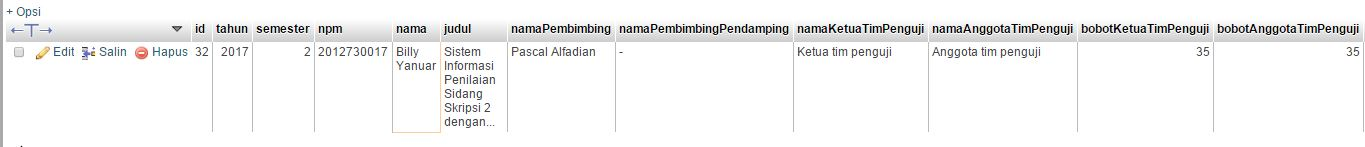
\includegraphics[scale=0.5]{Gambar/hasildatabase}
			\caption{Sebagian hasil pada database}
			\label{fig:hasildatabase}
		\end{figure}
	\end{enumerate}
	
\section{Hasil Pengujian}
\label{sec:hasilUji}

	Pengujian pada sistem informasi penilaian sidang skripsi 2 merupakan pengujian bersifat fungsional, dan pengujian eksperimental. Berikut penjelasannya:
	
	\subsection{Pengujian Eksperimental}
	\label{sub: PEksperimen}
	
	Pengujian eksperimental dilakukan dengan cara mengikuti sidang skripsi 2 yang dilakukan pada semester ganjil 2016/2017. Pada sidang yang diujikan, penilaian dilakukan dengan dua cara, yaitu dengan sistem kini yang bekerja secara manual dan dengan sistem usulan menggunakan laptop. Sehubungan dengan sifat kerasahasiaan \textit{data} pengujian, maka dengan persetujuan pembimbing pengujian eksperimental dilakukan dengan merahasiakan identitas mahasiswa yang berhubungan.
	
	Pada saat melakukan pengujian eksperimental, sistem kini memiliki kekurangan kecerobohan manusia yang mengakibatkan kesalahan dalam perhitungan nilai baik dari lembar rekapitulasi maupun lembar berita acara sidang skripsi. Hal tersebut diketahui pada saat membandingkan nilai perhitungan nilai akhir yang didapatkan oleh mahasiswa pada sistem kini dan sistem usulan. Pada beberapa kesalahan tersebut, penguji kembali melakukan perhitungan secara manual dengan menggunakan mesin hitung berupa kalkulator pada \textit{gadget} penguji. Setelah perhitungan dilakukan, didapatkan bahwa sistem usulan memiliki hasil yang benar.
	
	Percobaan eksperimental menghasilkan kesimpulan sistem usulan dapat menutupi kekurangan sistem kini yang berfokus pada perhitungan penilaian mahasiswa. Dengan menggunakan sistem usulan, perhitungan nilai dibuktikan lebih akurat dibandingkan dengan sistem kini.
	
	\subsection{Pengujian Fungsional}
	\label{sub: PFungsional}
	Pengujian fungsional dilakukan untuk mengetahui apakah sistem informasi dapat menjalankan seluruh fungsi-fungsi yang dimiliki dengan baik. Hasil pengujian fungsional sistem informasi akan dijabarkan pada tabel berikut:\\
	\begin{tabular}{| m{0.75cm} | m{7cm} | m{5cm} | m{3cm} |}
		\hline
		No & Aksi Pengguna & Reaksi yang diharapkan & Keterangan \\
		\hline
		1 & Pengguna menjalankan sistem informasi & Halaman berita acara ditampilkan & Reaksi sesuai \\
		\hline
		2 & Pengguna memasukkan nilai & Menampilkan hasil dari perhitungan otomatis & Reaksi sesuai \\
		\hline
		3 & Pengguna menekan tombol selesai & Menampilkan notifikasi data telah tersimpan & Reaksi sesuai \\
		\hline
		4 & Pengguna menekan tombol ok pada notifikasi & Menampilkan kembali halaman lembar formulir berita acara awal sebelum terisi & Reaksi sesuai \\
		\hline
	\end{tabular}}{}
\ifdefstring{\vbabf}{1}{\chapter{Kesimpulan dan Saran}
\label{chap: kesimpulan}

\section{Kesimpulan}
\label{sec: kesimpulan}
	
	Berdasarkan hasil penelitian yang dilakukan, didapatkan kesimpulan-kesimpulan sebagai berikut:
	\begin{enumerate}
		\item Penilaian skripsi terutama pada skripsi 2 masih menggunakan sistem manual, yaitu penilai mengisi dengan menuliskan nilai dan menghitung nilai akhir dengan alat hitung masing-masing pada lembar penilaian yang diberikan.
		\item Proses penyimpanan Sistem Informasi Penilaian Sidang Skripsi 2 dilakukan dengan menyimpan bobot dan nilai akhir yang telah dihitung secara otomatis oleh AngularJS.
		\item AngularJS bekerja dengan mengambil nilai input yang diperlukan dan melakukan perhitungan tanpa diperlukannya pergantian \textit{page} pada sistem penilaian, sehingga \textit{single page application} dapat terlaksana dengan maksimal pada sistem penilaian.
	\end{enumerate}

\section{Saran}
\label{sec: saran}

	Berdasarkan pengujian yang dilakukan, berikut adalah beberapa saran untuk pengembang:
	\begin{itemize}
		\item Menambahkan sistem manajemen nilai skripsi untuk melakukan fungsi \textit{select, update,} dan \textit{delete} karena Sistem Penilaian Sidang Skripsi 2 yang dibuat hanya menangani fungsi \textit{insert} ke \textit{database}.
	\end{itemize}
	}{}
\ifdefstring{\vbabg}{1}{\include{Bab/bab7}}{}
\ifdefstring{\vbabh}{1}{\include{Bab/bab8}}{}
\ifdefstring{\vbabi}{1}{\include{Bab/bab9}}{}

\bibliographystyle{ieeetr}
\bibliography{pustaka}

\appendix
\apptoc

\tampillmp{\vlmp}
\ifdefstring{\vlmpa}{1}{\chapter{Form Penilaian Skripsi}
\label{app:A}

Berikut adalah lembaran penilaian Skripsi yang di pakai di Program Studi Teknik Informatika Universitas Katolik Parahyangan~\ref{fig:appxa2}:

\begin{figure}[H]
\centering
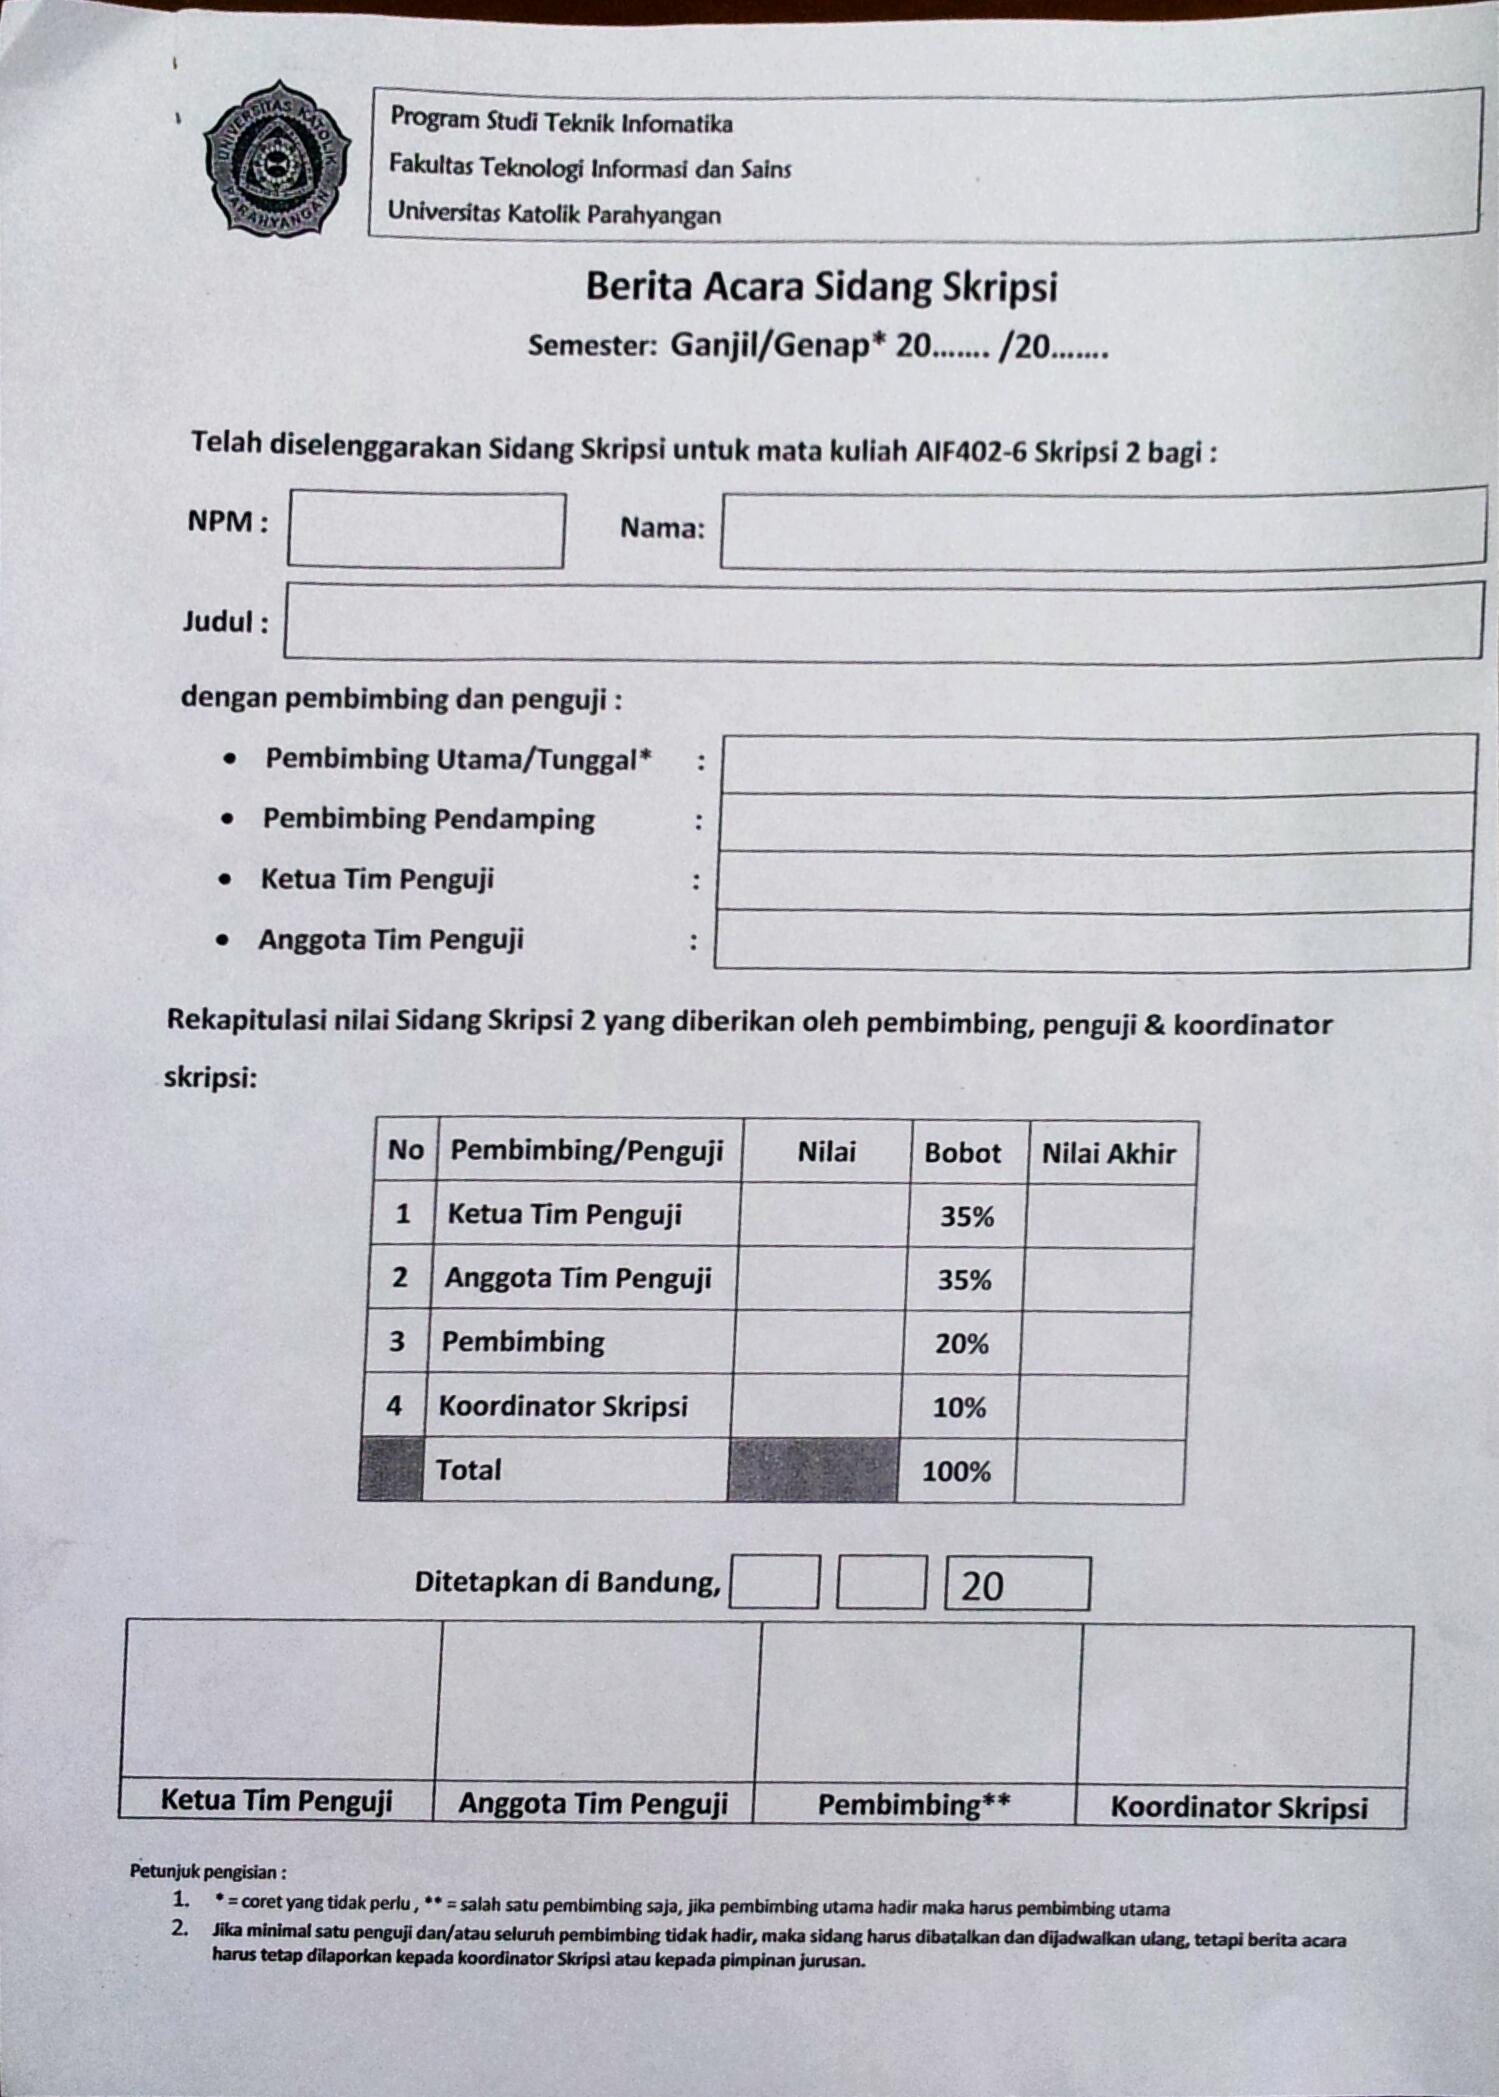
\includegraphics[scale=0.20]{Gambar/dokumen_skripsi}
\caption[Form Penilaian Skripsi saat sidang]{Form Penilaian Skripsi saat sidang} 
\label{fig: skripsiAsli}
\end{figure}
\pagebreak
Berikut adalah lembaran rekapitulasi penilaian Skripsi yang di pakai di Program Studi Teknik Informatika Universitas Katolik Parahyangan~\ref{fig:appxa3}:

\begin{figure}[H]
	\centering
	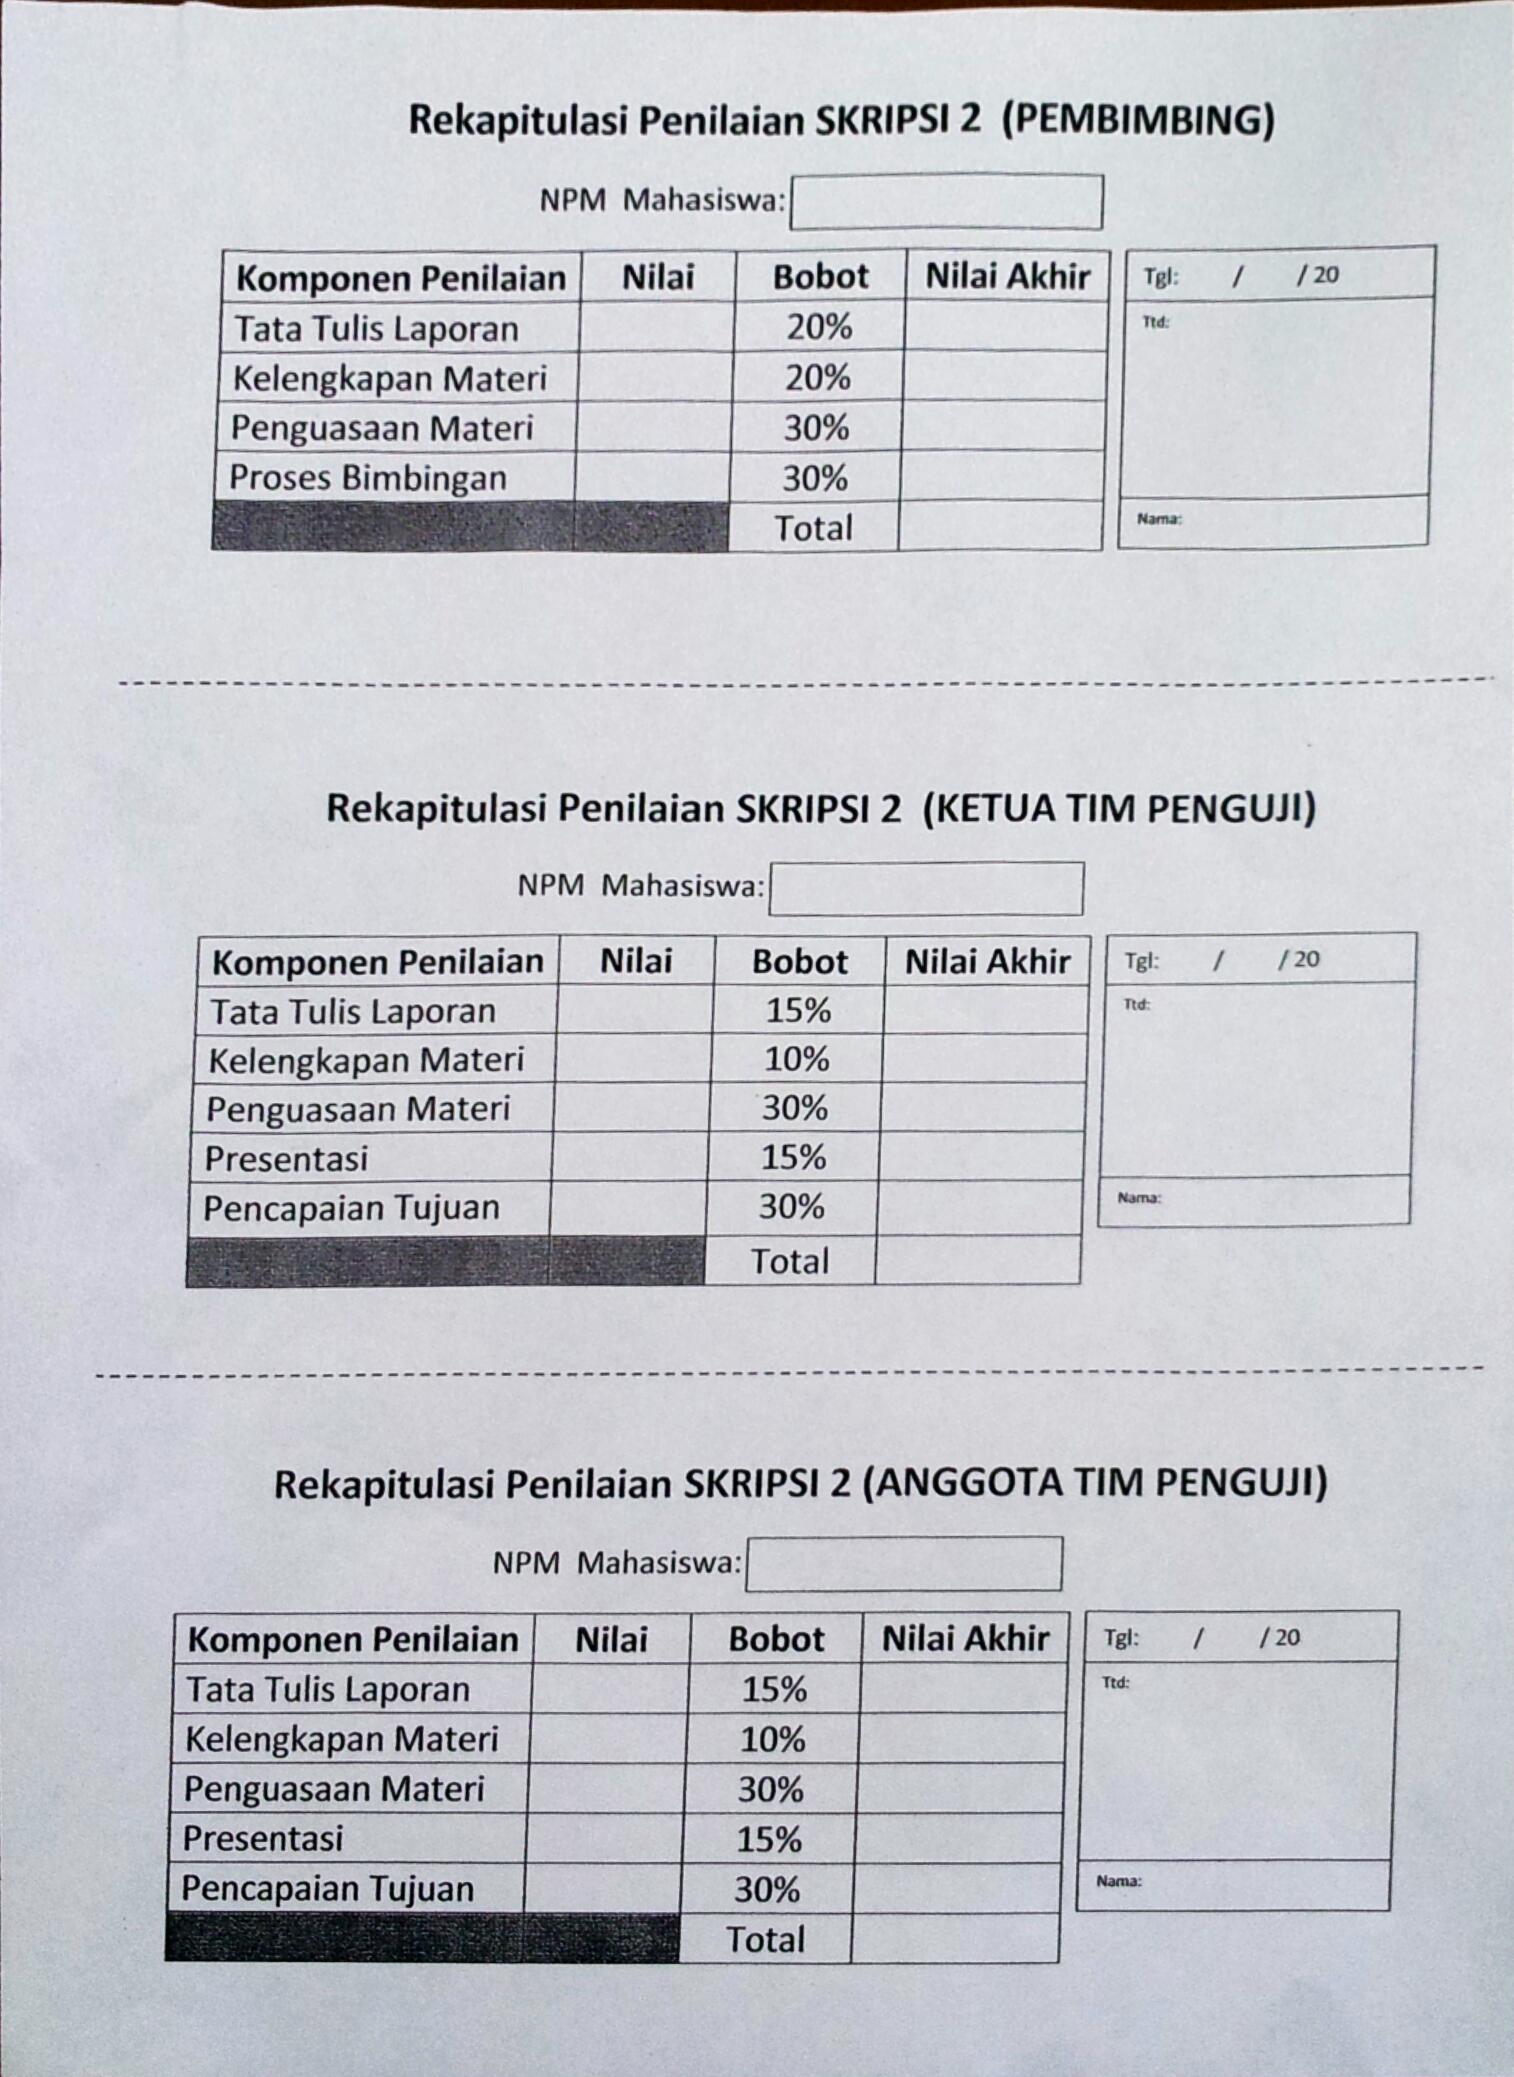
\includegraphics[scale=0.20]{Gambar/dokumen_rekap}
	\caption[Form Rekapitulasi Penilaian Skripsi saat sidang]{Form Rekapitulasi Penilaian Skripsi saat sidang} 
	\label{fig: rekapAsli}
\end{figure}}{}
\ifdefstring{\vlmpb}{1}{\chapter{The Source Code}
\label{app:B}

%selalu gunakan single spacing untuk source code !!!!!
\singlespacing 
% language: bahasa dari kode program
% terdapat beberapa pilihan : Java, C, C++, PHP, Matlab, R, dll
%
% basicstyle : ukuran font untuk kode program
% terdapat beberapa pilihan : tiny, scriptsize, footnotesize, dll
%
% caption : nama yang akan ditampilkan di dokumen akhir, lihat contoh
\begin{lstlisting}[language=PHP,basicstyle=\tiny,caption=C\_skripsi.php]
<?php
defined('BASEPATH') OR exit('No direct script access allowed');

class C_skripsi extends CI_Controller {

/**
* Index Page for this controller.
*
* Maps to the following URL
*              http://example.com/index.php/welcome
*      - or -
*              http://example.com/index.php/welcome/index
*      - or -
* Since this controller is set as the default controller in
* config/routes.php, it's displayed at http://example.com/
*
* So any other public methods not prefixed with an underscore will
* map to /index.php/welcome/<method_name>
* @see https://codeigniter.com/user_guide/general/urls.html
*/
	public function index()
	{
		$this->load->view('skripsi');
	}
	//Check database
	public function view_cekMahasiswa(){
		$data = $this->skripsi_model->getAllMahasiswa();
		$this->load->view('cek_mahasiswa', array('data' => $data));
	}
	
	public function tambahDataMahasiswa(){
		$semester = $_POST['semester'];
		$tahun = $_POST['tahun'];
		$npm = $_POST['npm'];
		$nama = $_POST['nama'];
		$judul = $_POST['judul'];
		$namaPembimbing = $_POST['namaPembimbing'];
		$namaPembimbingPendamping = $_POST['namaPembimbingPendamping'];
		$namaKetuaTimPenguji = $_POST['namaKetuaTimPenguji'];
		$namaAnggotaTimPenguji = $_POST['namaAnggotaTimPenguji'];
		$bobotKetuaTimPenguji = $_POST['bobotKetuaTimPenguji'];
		$bobotAnggotaTimPenguji = $_POST['bobotAnggotaTimPenguji'];
		$bobotPembimbing = $_POST['bobotPembimbing'];
		$nilaiKoordinatorSkripsi = $_POST['nilaiKoordinatorSkripsi'];
		$bobotKoordinatorSkripsi = $_POST['bobotKoordinatorSkripsi'];
		$bobotTataTulisLaporanAnggota = $_POST['bobotTataTulisLaporanAnggota'];
		$bobotKelengkapanMateriAnggota = $_POST['bobotKelengkapanMateriAnggota'];
		$bobotPenguasaanMateriAnggota = $_POST['bobotPenguasaanMateriAnggota'];
		$bobotPresentasiAnggota = $_POST['bobotPresentasiAnggota'];
		$bobotPencapaianTujuanAnggota = $_POST['bobotPencapaianTujuanAnggota'];
		$bobotTataTulisLaporanKetua = $_POST['bobotTataTulisLaporanKetua'];
		$bobotKelengkapanMateriKetua = $_POST['bobotKelengkapanMateriKetua'];
		$bobotPenguasaanMateriKetua = $_POST['bobotPenguasaanMateriKetua'];
		$bobotPresentasiKetua = $_POST['bobotPresentasiKetua'];
		$bobotPencapaianTujuanKetua = $_POST['bobotPencapaianTujuanKetua'];
		$bobotTataTulisLaporanPembimbing = $_POST['bobotTataTulisLaporanPembimbing'];
		$bobotKelengkapanMateriPembimbing = $_POST['bobotKelengkapanMateriPembimbing'];
		$bobotPenguasaanMateriPembimbing = $_POST['bobotPenguasaanMateriPembimbing'];
		$prosesBimbinganPembimbing = $_POST['prosesBimbinganPembimbing'];
		$nilaiAkhirMahasiswa = $_POST['nilaiAkhirMahasiswa'];
		$data_insert = array(
			'semester' => $semester,
			'tahun' => $tahun,
			'npm' => $npm,
			'nama' => $nama,
			'judul' => $judul,
			'namaPembimbing' => $namaPembimbing,
			'namaPembimbingPendamping' => $namaPembimbingPendamping,
			'namaKetuaTimPenguji' => $namaKetuaTimPenguji,
			'namaAnggotaTimPenguji' => $namaAnggotaTimPenguji,
			'bobotKetuaTimPenguji' => $bobotKetuaTimPenguji,
			'bobotAnggotaTimPenguji' => $bobotAnggotaTimPenguji,
			'bobotPembimbing' => $bobotPembimbing,
			'nilaiKoordinatorSkripsi' => $nilaiKoordinatorSkripsi,
			'bobotKoordinatorSkripsi' =>$bobotKoordinatorSkripsi,
			'bobotTataTulisLaporanAnggota' => $bobotTataTulisLaporanAnggota,
			'bobotKelengkapanMateriAnggota' => $bobotKelengkapanMateriAnggota,
			'bobotPenguasaanMateriAnggota' => $bobotPenguasaanMateriAnggota,
			'bobotPresentasiAnggota' => $bobotPresentasiAnggota,
			'bobotPencapaianTujuanAnggota' => $bobotPencapaianTujuanAnggota,
			'bobotTataTulisLaporanKetua' => $bobotTataTulisLaporanKetua,
			'bobotKelengkapanMateriKetua' => $bobotKelengkapanMateriKetua,
			'bobotPenguasaanMateriKetua' => $bobotPenguasaanMateriKetua,
			'bobotPresentasiKetua' => $bobotPresentasiKetua,
			'bobotPencapaianTujuanKetua' => $bobotPencapaianTujuanKetua,
			'bobotTataTulisLaporanPembimbing' => $bobotTataTulisLaporanPembimbing,
			'bobotKelengkapanMateriPembimbing' => $bobotKelengkapanMateriPembimbing,
			'bobotPenguasaanMateriPembimbing' => $bobotPenguasaanMateriPembimbing,
			'prosesBimbinganPembimbing' => $prosesBimbinganPembimbing,
			'nilaiAkhirMahasiswa' => $nilaiAkhirMahasiswa,
		
		);
		$res = $this->skripsi_model->insertDataMahasiswa('beritaacarasidangskripsi',$data_insert);
		redirect(base_url(), 'refresh');
	}

}

\end{lstlisting}

\begin{lstlisting}[language=PHP,basicstyle=\tiny,caption=skripsi.php]
<!DOCTYPE html>
<!--
To change this license header, choose License Headers in Project Properties.
To change this template file, choose Tools | Templates
and open the template in the editor.
-->
<html>
	<head>
		<meta charset="utf-8">
		<meta http-equiv="X-UA-Compatible" content="IE=edge">
		<meta name="viewport" content="width=device-width, initial-scale=1">
		<title> Berita Acara Sidang Skripsi </title>
		
		<!-- Bootstrap Core CSS -->
		<link href="public/css/bootstrap/bootstrap.min.css" rel="stylesheet">
		
		<!-- Custom Scroll Nav CSS -->
		<link href="public/css/scrolling-nav.css" rel="stylesheet">
		
		<!-- Custom CSS -->
		<link href="public/css/custom.css" rel="stylesheet">
		
		<!-- AngularJS -->
		<script src="public/js/angularJS/angular.min.js"></script>
		
		<!-- Mobile friendly bootstrap -->
		
		
	</head>
	<body ng-app="penilaian" id="page-top" data-spy="scroll" data-target=".navbar-fixed-top">
	
	
		<!-- Navigation -->
		<nav class="navbar navbar-default navbar-fixed-top" role="navigation">
			<div class="container">
				<div class="navbar-header page-scroll">
					<button type="button" class="navbar-toggle" data-toggle="collapse" data-target=".navbar-ex1-collapse">
						<span class="sr-only">Toggle navigation</span>
						<span class="icon-bar"></span>
						<span class="icon-bar"></span>
						<span class="icon-bar"></span>
					</button>
				</div>
				
				<form role="form" method="post" accept-charset="utf-8" action="<?php echo base_url() . "index.php/c_skripsi/tambahDataMahasiswa" ?>" ng-controller="DefaultValue">
					
					
					<!-- Collect the nav links, forms, and other content for toggling -->
					<div class="collapse navbar-collapse navbar-ex1-collapse">
						<ul class="nav navbar-nav">
							<!-- Hidden li included to remove active class from about link when scrolled up past about section -->
							<li>
								<a class="page-scroll" href="#page-top">Berita Acara Sidang Skripsi</a>
							</li>
							<li>
								<a class="page-scroll" href="#rekAnggota">Lembar Rekapitulasi Anggota Tim Penguji</a>
							</li>
							<li>
								<a class="page-scroll" href="#rekKetua">Lembar Rekapitulasi Ketua Tim Penguji</a>
							</li>
							<li>
								<a class="page-scroll" href="#rekPembimbing">Lembar Rekapitulasi Pembimbing</a>
							</li>
							<li>
								<a class="page-scroll" href="#selesai">Selesai</a>
							</li>
						</ul>
					</div>
					<!-- /.navbar-collapse -->
				</div>
				<!-- /.container -->
			</nav>
			
			
			
			<!-- Berita Acara Sidang Skripsi -->
			<section id="intro" class="intro-section">
				<!-- Page Heading -->
				<div class="container">
					<div class="row">
						<div class="col-lg-12">
							<div class="page-header">
								<h1>
									Berita Acara Sidang Skripsi
								</h1>
							
								<div class="semester">
									<p> 
									<label>Semester:</label>
									<!-- 1 -->
									<select name="semester">
										<option value="1">Ganjil</option>
										<option value="2">Genap</option>
									</select>
									<!-- 2 -->
									<input id="tahun" type="number" max="9999" ng-model="tahun" name="tahun"/>
									/
									<input id="tahun_1" type="number" max="9999" value="{{tahun + 1}}" disabled="disabled"/>
									
									</p>
								</div>
							</div>
						</div>
					</div>
				<!-- Isi -->
				<div class="row">
					<div class="col-lg-12">
					
						<div class="form-group">
						Telah diselenggarakan Sidang Skripsi untuk mata kuliah AIF402-6 Skripsi 2 bagi:
						
							<div id="pengenalMahasiswa">
								<p>
								<!-- 3 -->
								<label class="col-md-1 col-xs-6" for="npm">NPM:</label><input maxlength="10" id="npm" class="inline-form col-md-3 col-xs-6" ng-model="n_npm" name="npm"/>
								<!-- 4 -->
								<label class="col-md-1 col-xs-6" for="nama">Nama:</label><input id="nama" class="inline-form col-md-7 col-xs-6" name="nama"/>
								</p>
							</div>
							<br/>
							<div id="pengenalJudul">
								<p>
								<!-- 5 -->
								<label class="col-md-1 col-xs-6" for="judul">Judul:</label><input id="judul" class="inline-form col-md-11 col-xs-6" name="judul"/>
								</p>
							</div>
						</div>
					
						<p> dengan pembimbing dan penguji:</p>
					
					
						<div id="pengenalPembimbing">
							<p>
							<label class="col-md-3 col-xs-8" for="pembimbing">Pembimbing:</label>
							<!-- 6 -->
							<input class="col-md-9 col-xs-4" id="pembimbing" name="namaPembimbing"/>
							</p>
						</div>
						<br/>
					
						<div id="pengenalPembimbingPendamping">
							<p>
							<label class="col-md-3 col-xs-8" for="pembimbing2">Pembimbing Pendamping:</label>
							<!-- 7 -->
							<input class="col-md-9 col-xs-4" id="pembimbing2" name="namaPembimbingPendamping"/>
							</p>
						</div>
						<br/>
						<div id="pengenalKetua">
							<p>
							<label class="col-md-3 col-xs-8" for="ketua">Ketua Tim Penguji:</label>
							<!-- 8 -->
							<input class="col-md-9 col-xs-4" id="ketua" name="namaKetuaTimPenguji"/>
							
							</p>
						</div>
						<br/>
					
						<div id="pengenalAnggota">
							<p>
							<label class="col-md-3 col-xs-8" for="anggota">Anggota Tim Penguji:</label>
							<!-- 9 -->
							<input class="col-md-9 col-xs-4" id="anggota" name="namaAnggotaTimPenguji" />
							
							</p>
						</div>
						<br/>
						<p>Rekapitulasi nilai Sidang Skripsi 2 yang diberikan oleh pembimbing, penguji & koordinator skripsi:</p>
						<table class="col-md-8 col-xs-12 col-md-offset-4 col-md-pull-2 table-responsive">
							<tr>
								<th>No</th>
								<th>Pembimbing/Penguji</th>
								<th>Nilai</th>
								<th>Bobot(%)</th>
								<th>Nilai Akhir</th>
							</tr>
							<tr>
								<td>1</td>
								<td><label for="nKetua">Ketua Tim Penguji</label></td>
								<td><input type="number" id="nKetua" max="100" ng-model="nilai_ketua" class="form-nilai" value="{{nilai_TTLaporanK * TTLaporanK.value / 100 + nilai_KMateriK * KMateriK.value / 100 + nilai_PMateriK * PMateriK.value / 100 + nilai_PresentasiK * presentasiK.value / 100 + nilai_PTujuanK * PTujuanK.value / 100}}" disabled="disabled" /></td>
								<!-- 10 -->
								<td><input type="number" ng-model="ketua.value" ng-init="ketua.value = 35" min="0" max="100" class="form-nilai" name="bobotKetuaTimPenguji" readonly="readonly" /></td>
								<td><input type="number" value="{{(nilai_TTLaporanK * TTLaporanK.value / 100 + nilai_KMateriK * KMateriK.value / 100 + nilai_PMateriK * PMateriK.value / 100 + nilai_PresentasiK * presentasiK.value / 100 + nilai_PTujuanK * PTujuanK.value / 100) * ketua.value / 100}}" ng-model="total_ketua" class="form-nilai" disabled="disabled" /></td>
							</tr>
							<tr>
								<td>2</td>
								<td><label for="nAnggota">Anggota Tim Penguji</label></td>
								<td><input id="nAnggota" type="number" max="100" ng-model="nilai_anggota" class="form-nilai" value="{{nilai_TTLaporanA * TTLaporanA.value / 100 + nilai_KMateriA * KMateriA.value / 100 + nilai_PMateriA * PMateriA.value / 100 + nilai_PresentasiA * presentasiA.value / 100 + nilai_PTujuanA * PTujuanA.value / 100}}" disabled="disabled" /></td>
								<!-- 11 -->
								<td><input type="number" ng-model="anggota.value" ng-init="anggota.value = 35" min="0" max="100" class="form-nilai" name="bobotAnggotaTimPenguji" readonly="readonly" /></td>
								<td><input type="number" value="{{(nilai_TTLaporanA * TTLaporanA.value / 100 + nilai_KMateriA * KMateriA.value / 100 + nilai_PMateriA * PMateriA.value / 100 + nilai_PresentasiA * presentasiA.value / 100 + nilai_PTujuanA * PTujuanA.value / 100) * anggota.value / 100}}" ng-model="total_anggota" class="form-nilai" disabled="disabled" /></td>
							</tr>
							<tr>
								<td>3</td>
								<td><label for="nPembimbing">Pembimbing</label></td>
								<td><input id="nPembimbing" type="number" max="100" ng-model="nilai_pembimbing" class="form-nilai" min=0 value="{{nilai_TTLaporanP * TTLaporanP.value / 100 + nilai_KMateriP * KMateriP.value / 100 + nilai_PMateriP * PMateriP.value / 100 + nilai_PBimbinganP * PBimbinganP.value / 100}}" disabled="disabled" /></td>
								<!-- 12 -->
								<td><input type="number" ng-model="pembimbing.value" ng-init="pembimbing.value = 20" min="0" max="100" class="form-nilai" name="bobotPembimbing" readonly="readonly" /></td>
								<td><input type="number" value="{{(nilai_TTLaporanP * TTLaporanP.value / 100 + nilai_KMateriP * KMateriP.value / 100 + nilai_PMateriP * PMateriP.value / 100 + nilai_PBimbinganP * PBimbinganP.value / 100) * pembimbing.value / 100}}" ng-model="total_pembimbing" class="form-nilai" disabled="disabled" /></td>
							</tr>
							<tr>
								<td>4</td>
								<td><label for="nKoordinator">Koordinator Skripsi</label></td>
								<!-- 13 -->
								<td><input id="nKoordinator" type="number" max="100" ng-model="nilai_koordinator" class="form-nilai" min=0 name="nilaiKoordinatorSkripsi"/></td>
								<!-- 14 -->
								<td><input type="number"  ng-model="koordinator.value" ng-init="koordinator.value = 10" min="0" max="100" class="form-nilai" name="bobotKoordinatorSkripsi" readonly="readonly" /></td>
								<td><input type="number" value={{nilai_koordinator*koordinator.value/100}} ng-model="total_koodinator" class="form-nilai" disabled="disabled" /></td>
							</tr>
							<tr>
								<td></td>
								<td colspan="2" ><label for="nTotal">Total</label></td>
								<td><input type="number" id="nTotal" max="100" disabled="disabled" value={{ketua.value+anggota.value+pembimbing.value+koordinator.value}} class="form-nilai"/></td>
								<!-- 29 -->
								<td><input type="number" name="nilaiAkhirMahasiswa" value= "{{(nilai_TTLaporanK * TTLaporanK.value / 100 + nilai_KMateriK * KMateriK.value / 100 + nilai_PMateriK * PMateriK.value / 100 + nilai_PresentasiK * presentasiK.value / 100 + nilai_PTujuanK * PTujuanK.value / 100 )* ketua.value / 100 + (nilai_TTLaporanA * TTLaporanA.value / 100 + nilai_KMateriA * KMateriA.value / 100 + nilai_PMateriA * PMateriA.value / 100 + nilai_PresentasiA * presentasiA.value / 100 + nilai_PTujuanA * PTujuanA.value / 100) * anggota.value / 100 + (nilai_TTLaporanP * TTLaporanP.value / 100 + nilai_KMateriP * KMateriP.value / 100 + nilai_PMateriP * PMateriP.value / 100 + nilai_PBimbinganP * PBimbinganP.value / 100) * pembimbing.value / 100 + nilai_koordinator * koordinator.value / 100}}" class="form-nilai"/></td>
							</tr>
						</table>
					</div> 
				</div>
			</section>
			
			
			
			
			<!-- Rekapitulasi Ketua Tim Penguji -->
			<section id="rekKetua" class="rekKetua-section">
				<!-- Page Heading -->
				<div class="container">
					<div class="row">
						<div class="col-lg-6.col-lg-offset-3">
							<div class="page-header">
								<h1>
									Rekapitulasi Penilaian Skripsi 2 (Ketua Tim Penguji)
								</h1>
								<div class="semester">
									<p> 
									<label for="npmK">NPM:</label><input id="nmpK" maxlength="10" value="{{ n_npm}}" disabled="disabled" />
									</p>
								</div>
							</div>
						</div>
					</div>
					<!-- Isi Rekapitulasi Ketua Tim Penguji -->
					<div class="row">
						<div class="col-lg-12">
							<table class="col-md-8 col-xs-12 col-md-offset-4 col-md-pull-2 table-responsive">
								<tr>
									<th>Komponen Penilaian</th>
									<th>Nilai</th>
									<th>Bobot(%)</th> 
									<th>Nilai Akhir</th>
								</tr>
								<tr>
									<td><label for="nTTLaporanK">Tata Tulis Laporan</label></td>
									<td><input type="number" id="nTTLaporanK" max="100" ng-model="nilai_TTLaporanK" class="form-nilai"/></td>
									<!-- 20 -->
									<td><input type="number" name="bobotTataTulisLaporanKetua" ng-model="TTLaporanK.value" ng-init="TTLaporanK.value = 15" min="0" max="100" class="form-nilai" readonly="readonly" /></td>
									<td><input type="number" disabled="disabled" value="{{nilai_TTLaporanK * TTLaporanK.value / 100}}" ng-model="total_TTLaporanK" class="form-nilai"/></td>
								</tr>
								<tr>
									<td><label for="nKMateriK">Kelengkapan Materi</label></td>
									<td><input type="number" id="nKMateriK" max="100" ng-model="nilai_KMateriK" class="form-nilai"/></td>
									<!-- 21 -->
									<td><input type="number" name="bobotKelengkapanMateriKetua" ng-model="KMateriK.value" ng-init="KMateriK.value = 10" min="0" max="100" class="form-nilai" readonly="readonly" /></td>
									<td><input type="number" disabled="disabled" value="{{nilai_KMateriK * KMateriK.value / 100}}" ng-model="total_KMateriK" class="form-nilai"/></td>
								</tr>
								<tr>
									<td><label for="nPMateriK">Penguasaan Materi</label></td>
									<td><input type="number" id="nPMateriK" max="100" ng-model="nilai_PMateriK" class="form-nilai"/></td>
									<!-- 22 -->
									<td><input type="number" name="bobotPenguasaanMateriKetua" ng-model="PMateriK.value" ng-init="PMateriK.value = 30" min="0" max="100" class="form-nilai" readonly="readonly" /></td>
									<td><input type="number" disabled="disabled" value="{{nilai_PMateriK * PMateriK.value / 100}}" ng-model="total_PMateriA" class="form-nilai"/></td>
								</tr>
								<tr>
									<td><label for="nPresentasiK">Presentasi</label></td>
									<td><input type="number" id="nPresentasiK" max="100" ng-model="nilai_PresentasiK" class="form-nilai"/></td>
									<!-- 23 -->
									<td><input type="number" name="bobotPresentasiKetua" ng-model="presentasiK.value" ng-init="presentasiK.value = 15" min="0" max="100" class="form-nilai" readonly="readonly" /></td>
									<td><input type="number" disabled="disabled" value="{{nilai_PresentasiK * presentasiK.value / 100}}" ng-model="total_PresentasiK" class="form-nilai"/></td>
								</tr>
								<tr>
									<td><label for="nPTujuanK">Pencapaian Tujuan</label></td>
									<td><input type="number" id="nPTujuanK" max="100" ng-model="nilai_PTujuanK" class="form-nilai"/></td>
									<!-- 24 -->
									<td><input type="number" name="bobotPencapaianTujuanKetua" ng-model="PTujuanK.value" ng-init="PTujuanK.value = 30" min="0" max="100" class="form-nilai" readonly="readonly" /></td>
									<td><input type="number" disabled="disabled" value="{{nilai_PTujuanK * PTujuanK.value / 100}}" ng-model="total_PTujuanK" class="form-nilai"/></td>
								</tr>
								<tr>
									<td colspan="2" ><label for="nTotalBobotK">Total</label></td>
									<td><input type="number" id="nTotalBobotK" max="100" disabled="disabled" value={{TTLaporanK.value+KMateriK.value+PMateriK.value+presentasiK.value+PTujuanK.value}} class="form-nilai"/></td>
									<td><input type="number" id="nTotalKetua" ng-model="nTotalKetua" max="100" value= "{{nilai_TTLaporanK * TTLaporanK.value / 100 + nilai_KMateriK * KMateriK.value / 100 + nilai_PMateriK * PMateriK.value / 100 + nilai_PresentasiK * presentasiK.value / 100 + nilai_PTujuanK * PTujuanK.value / 100}}" class="form-nilai" disabled="disabled" /></td>
								</tr>
							</table>
						</div>
					</div>
				</div>
			</section>
			
			<!-- Rekapitulasi Anggota Tim Penguji -->
			<section id="rekAnggota" class="rekAnggota-section">
				<!-- Page Heading -->
				<div class="container">
					<div class="row">
						<div class="col-lg-6.col-lg-offset-3">
							<div class="page-header">
								<h1>
								Rekapitulasi Penilaian Skripsi 2 (Anggota Tim Penguji)
								</h1>
								<div class="semester">
									<p> 
									<label for="npmA">NPM:</label><input id="nmpA" maxlength="10" value="{{ n_npm}}" disabled="disabled" />
									</p>
								</div>
							</div>
						</div>
					</div>
					<!-- Isi Rekapitulasi Anggota Tim Penguji -->
					<div class="row">
						<div class="col-lg-12">
							<table class="col-md-8 col-xs-12 col-md-offset-4 col-md-pull-2 table-responsive">
								<tr>
									<th>Komponen Penilaian</th>
									<th>Nilai</th>
									<th>Bobot(%)</th>
									<th>Nilai Akhir</th>
								</tr>
								<tr>
									<td><label for="nTTLaporanA">Tata Tulis Laporan</label></td>
									<td><input type="number" id="nTTLaporanA" max="100" ng-model="nilai_TTLaporanA" class="form-nilai"/></td>
									<!-- 15 -->
									<td><input type="number" name="bobotTataTulisLaporanAnggota" ng-model="TTLaporanA.value" ng-init="TTLaporanA.value = 15" min="0" max="100" class="form-nilai" readonly="readonly" /></td>
									<td><input type="number" disabled="disabled" value="{{nilai_TTLaporanA * TTLaporanA.value / 100}}" ng-model="total_TTLaporanA" class="form-nilai"/></td>
								</tr>
								<tr>
									<td><label for="nKMateriA">Kelengkapan Materi</label></td>
									<td><input type="number" id="nKMateriA" max="100" ng-model="nilai_KMateriA" class="form-nilai"/></td>
									<!-- 16 -->
									<td><input type="number" name="bobotKelengkapanMateriAnggota" ng-model="KMateriA.value" ng-init="KMateriA.value = 10" min="0" max="100" class="form-nilai" readonly="readonly" /></td>
									<td><input type="number" disabled="disabled" value="{{nilai_KMateriA * KMateriA.value / 100}}" ng-model="total_KMateriA" class="form-nilai"/></td>
								</tr>
								<tr>
									<td><label for="nPMateriA">Penguasaan Materi</label></td>
									<td><input type="number" id="nPMateriA" max="100" ng-model="nilai_PMateriA" class="form-nilai"/></td>
									<!-- 17 -->
									<td><input type="number" name="bobotPenguasaanMateriAnggota" ng-model="PMateriA.value"  ng-init="PMateriA.value = 30" min="0" max="100" class="form-nilai" readonly="readonly" /></td>
									<td><input type="number" disabled="disabled" value="{{nilai_PMateriA * PMateriA.value / 100}}" ng-model="total_PMateriA" class="form-nilai"/></td>
								</tr>
								<tr>
									<td><label for="nPresentasiA">Presentasi</label></td>
									<td><input type="number" id="nPresentasiA" max="100" ng-model="nilai_PresentasiA" class="form-nilai"/></td>
									<!-- 18 -->
									<td><input type="number" name="bobotPresentasiAnggota" ng-model="presentasiA.value" ng-init="presentasiA.value = 15" min="0" max="100" class="form-nilai" readonly="readonly" /></td>
									<td><input type="number" disabled="disabled" value="{{nilai_PresentasiA * presentasiA.value / 100}}" ng-model="total_PresentasiA" class="form-nilai"/></td>
								</tr>
								<tr>
									<td><label for="nPTujuanA">Pencapaian Tujuan</label></td>
									<td><input type="number" id="nPTujuanA" max="100" ng-model="nilai_PTujuanA" class="form-nilai"/></td>
									<!-- 19 -->
									<td><input type="number" name="bobotPencapaianTujuanAnggota" ng-model="PTujuanA.value" ng-init="PTujuanA.value = 30" min="0" max="100" class="form-nilai" readonly="readonly" /></td>
									<td><input type="number" disabled="disabled" value="{{nilai_PTujuanA * PTujuanA.value / 100}}" ng-model="total_PTujuanA" class="form-nilai"/></td>
								</tr>
								<tr>
									<td colspan="2" ><label for="nTotalBobotA">Total</label></td>
									<td><input type="number" id="nTotalBobotA" max="100" disabled="disabled" value={{TTLaporanA.value+KMateriA.value+PMateriA.value+presentasiA.value+PTujuanA.value}} class="form-nilai"/></td>
									<td><input type="number" id="nTotalAnggota" ng-model="nTotalAnggota" max="100" class="form-nilai" value= "{{nilai_TTLaporanA * TTLaporanA.value / 100 + nilai_KMateriA * KMateriA.value / 100 + nilai_PMateriA * PMateriA.value / 100 + nilai_PresentasiA * presentasiA.value / 100 + nilai_PTujuanA * PTujuanA.value / 100}}" disabled="disabled" /></td>
								</tr>
							</table>
							
						</div>
					</div>
				</div>
			</section>
			
			<!-- Rekapitulasi Pembimbing -->
			<section id="rekPembimbing" class="rekPembimbing-section">
				<!-- Page Heading -->
				<div class="container">
					<div class="row">
						<div class="col-lg-6.col-lg-offset-3">
							<div class="page-header">
							<h1>
							Rekapitulasi Penilaian Skripsi 2 (Pembimbing)
							</h1>
								<div class="semester">
									<p> 
									<label for="npmP">NPM:</label><input id="nmpP" maxlength="10" value="{{ n_npm}}" disabled="disabled" />
									</p>
								</div>
							</div>
						</div>
					</div>
					<!-- Isi Rekapitulasi Pembimbing -->
					<div class="row">
						<div class="col-lg-12">
							<table class="col-md-8 col-xs-12 col-md-offset-4 col-md-pull-2 table-responsive">
								<tr>
									<th>Komponen Penilaian</th>
									<th>Nilai</th>
									<th>Bobot(%)</th>
									<th>Nilai Akhir</th>
								</tr>
								<tr>
									<td><label for="nTTLaporanP">Tata Tulis Laporan</label></td>
									<td><input type="number" id="nTTLaporanP" max="100" ng-model="nilai_TTLaporanP" class="form-nilai"/></td>
									<!-- 25 -->
									<td><input type="number" name="bobotTataTulisLaporanPembimbing" ng-model="TTLaporanP.value" ng-init="TTLaporanP.value = 20" min="0" max="100" class="form-nilai" readonly="readonly" /></td>
									<td><input type="number" disabled="disabled" value="{{nilai_TTLaporanP * TTLaporanP.value / 100}}" ng-model="total_TTLaporanP" class="form-nilai"/></td>
								</tr>
								<tr>
									<td><label for="nKMateriP">Kelengkapan Materi</label></td>
									<td><input type="number" id="nKMateriP" max="100" ng-model="nilai_KMateriP" class="form-nilai"/></td>
									<!-- 26 -->
									<td><input type="number" name="bobotKelengkapanMateriPembimbing" ng-model="KMateriP.value" ng-init="KMateriP.value = 20" min="0" max="100" class="form-nilai" readonly="readonly" /></td>
									<td><input type="number" disabled="disabled" value="{{nilai_KMateriP * KMateriP.value / 100}}" ng-model="total_KMateriP" class="form-nilai"/></td>
								</tr>
								<tr>
									<td><label for="nPMateriP">Penguasaan Materi</label></td>
									<td><input type="number" id="nPMateriP" max="100" ng-model="nilai_PMateriP" class="form-nilai"/></td>
									<!-- 27 -->
									<td><input type="number" name="bobotPenguasaanMateriPembimbing" ng-model="PMateriP.value" ng-init="PMateriP.value = 30" min="0" max="100" class="form-nilai" readonly="readonly" /></td>
									<td><input type="number" disabled="disabled" value="{{nilai_PMateriP * PMateriP.value / 100}}" ng-model="total_PMateriP" class="form-nilai"/></td>
								</tr>
								<tr>
									<td><label for="nPBimbinganP">Proses Bimbingan</label></td>
									<td><input type="number" id="nPBimbinganP" max="100" ng-model="nilai_PBimbinganP" class="form-nilai"/></td>
									<!-- 28 -->
									<td><input type="number" name="prosesBimbinganPembimbing" ng-model="PBimbinganP.value" ng-init="PBimbinganP.value = 30" min="0" max="100" class="form-nilai" readonly="readonly" /></td>
									<td><input type="number" disabled="disabled" value="{{nilai_PBimbinganP * PBimbinganP.value / 100}}" ng-model="total_PBimbinganP" class="form-nilai"/></td>
								</tr>
								<tr>
									<td colspan="2" ><label for="nTotalBobotP">Total</label></td>
									<td><input type="number" id="nTotalBobotP" max="100" disabled="disabled" value={{TTLaporanP.value+KMateriP.value+PMateriP.value+PBimbinganP.value}} class="form-nilai"/></td>
									<td><input type="number" id="nTotalPembimbing" ng-model="nTotalPembimbing" max="100"  value= "{{nilai_TTLaporanP * TTLaporanP.value / 100 + nilai_KMateriP * KMateriP.value / 100 + nilai_PMateriP * PMateriP.value / 100 + nilai_PBimbinganP * PBimbinganP.value / 100}}" class="form-nilai" disabled="disabled" /></td>
								</tr>
							</table>
						</div>
					</div>
				</div>
			</section>
			
			<!-- Selesai -->
			<section id="selesai" class="rekPembimbing-section">
				<!-- Page Heading -->
				<div class="container">
					<div class="row">
						<div class="col-lg-6.col-lg-offset-3">
							<div class="page-header">
								<div class= "tanggal">
								<p>
								Ditetapkan di Bandung, <span id="date"></span>
								</p>
								
								
								<script>
								var months = ['Januari', 'Februari', 'Maret', 'April', 'Mei', 'Juni', 'Juli', 'Agustus', 'September', 'Oktober', 'November', 'Desember'];
								var myDays = ['Minggu', 'Senin', 'Selasa', 'Rabu', 'Kamis', 'Jum&#39;at', 'Sabtu'];
								var date = new Date();
								var day = date.getDate();
								var month = date.getMonth();
								var thisDay = date.getDay(),
								thisDay = myDays[thisDay];
								var yy = date.getYear();
								var year = (yy < 1000) ? yy + 1900 : yy;
								
								
								newdate = thisDay + ', ' + day + ' ' + months[month] + ' ' + year;
								document.getElementById("date").innerHTML = newdate;
								
								newyear = parseInt(year);
								document.getElementById("tahun").value = newyear;
								</script>
								<p><input type="submit" name="submit" value="Selesai"></p>
								</div>
							</div>
						</div>
					</div>
				</div>
			</section>	
		</form>
		<!-- Set Default Value pada ng-model type number -->
		<script>
		angular.module('penilaian', [])
		.controller('DefaultValue', ['$scope', function ($scope) {
		
		}]);
		</script>
		
		<!-- jQuery -->
		<script src="public/js/jQuery/jquery.min.js"></script>
		
		<!-- Bootstrap Core JavaScript -->
		<script src="public/js/bootstrap/bootstrap.min.js"></script>
		
		<!-- Scrolling Nav JavaScript -->
		<script src="public/js/jquery.easing.min.js"></script>
		<script src="public/js/scrolling-nav.js"></script>
		
	</body>
</html>
\end{lstlisting}

\begin{lstlisting}[language=PHP,basicstyle=\tiny,caption=skripsi\_model.php]
<?php
defined('BASEPATH') OR exit('No direct script access allowed');

class Skripsi_model extends CI_Model {

	public function insertDataMahasiswa($tableName, $data){
		$res = $this->db->insert($tableName, $data);
	}
	
	public function getAllMahasiswa(){
		$query = $this->db->get('beritaacarasidangskripsi');
		return $query->result_array();
	}
}

\end{lstlisting}
\begin{lstlisting}[language=PHP,basicstyle=\tiny,caption=scrolling-nav.css]
/*!
* Start Bootstrap - Scrolling Nav HTML Template (http://startbootstrap.com)
* Code licensed under the Apache License v2.0.
* For details, see http://www.apache.org/licenses/LICENSE-2.0.
*/

body {
	width: 100%;
	height: 100%;
}

html {
	width: 100%;
	height: 100%;
}

@media(min-width:767px) {
	.navbar {
	padding: 20px 0;
	-webkit-transition: background .5s ease-in-out,padding .5s ease-in-out;
	-moz-transition: background .5s ease-in-out,padding .5s ease-in-out;
	transition: background .5s ease-in-out,padding .5s ease-in-out;
	}
	
	.top-nav-collapse {
		padding: 0;
	}
}

/* Demo Sections - You can use these as guides or delete them - the scroller will work with any sort of height, fixed, undefined, or percentage based.
The padding is very important to make sure the scrollspy picks up the right area when scrolled to. Adjust the margin and padding of sections and children 
of those sections to manage the look and feel of the site. */

.intro-section {
	height: 100%;
	padding-top: 80px;
	background: #fff;
}
\end{lstlisting}

\begin{lstlisting}[language=PHP,basicstyle=\tiny,caption=custom.css]
/* My Custom CSS */
.form-nilai{
	width: 45px;
}

.page-header{
	text-align: center;
}
tr{
	height:30px;
}
.rekAnggota-section {
	height: 100%;
	padding-top: 80px;
	background: #fff;
}

.rekKetua-section {
	height: 100%;
	padding-top: 80px;
	background: #fff;
}

.rekPembimbing-section {
	height: 100%;
	padding-top: 80px;
	background: #fff;
}
input[disabled="disabled"]{
	background-color: #fff;
}

\end{lstlisting}

\begin{lstlisting}[language=PHP,basicstyle=\tiny,caption=scrolling-nav.js]
//jQuery to collapse the navbar on scroll
$(window).scroll(function() {
	if ($(".navbar").offset().top > 50) {
	$(".navbar-fixed-top").addClass("top-nav-collapse");
	} else {
	$(".navbar-fixed-top").removeClass("top-nav-collapse");
	}
});

//jQuery for page scrolling feature - requires jQuery Easing plugin
$(function() {
	$('a.page-scroll').bind('click', function(event) {
		var $anchor = $(this);
		$('html, body').stop().animate({
		scrollTop: $($anchor.attr('href')).offset().top
		}, 1500, 'easeInOutExpo');
		event.preventDefault();
	});
});

\end{lstlisting}}{}
\ifdefstring{\vlmpc}{1}{\chapter{Form Revisi}
\label{chap: revisi}

Gambar \ref{fig: revisi} adalah lembaran yang digunakan sebagai penanda revisi yang harus dilakukan pada skripsi Sistem Penilaian Sidang Skripsi2 dengan AngularJS:

\begin{figure}[H]
\centering
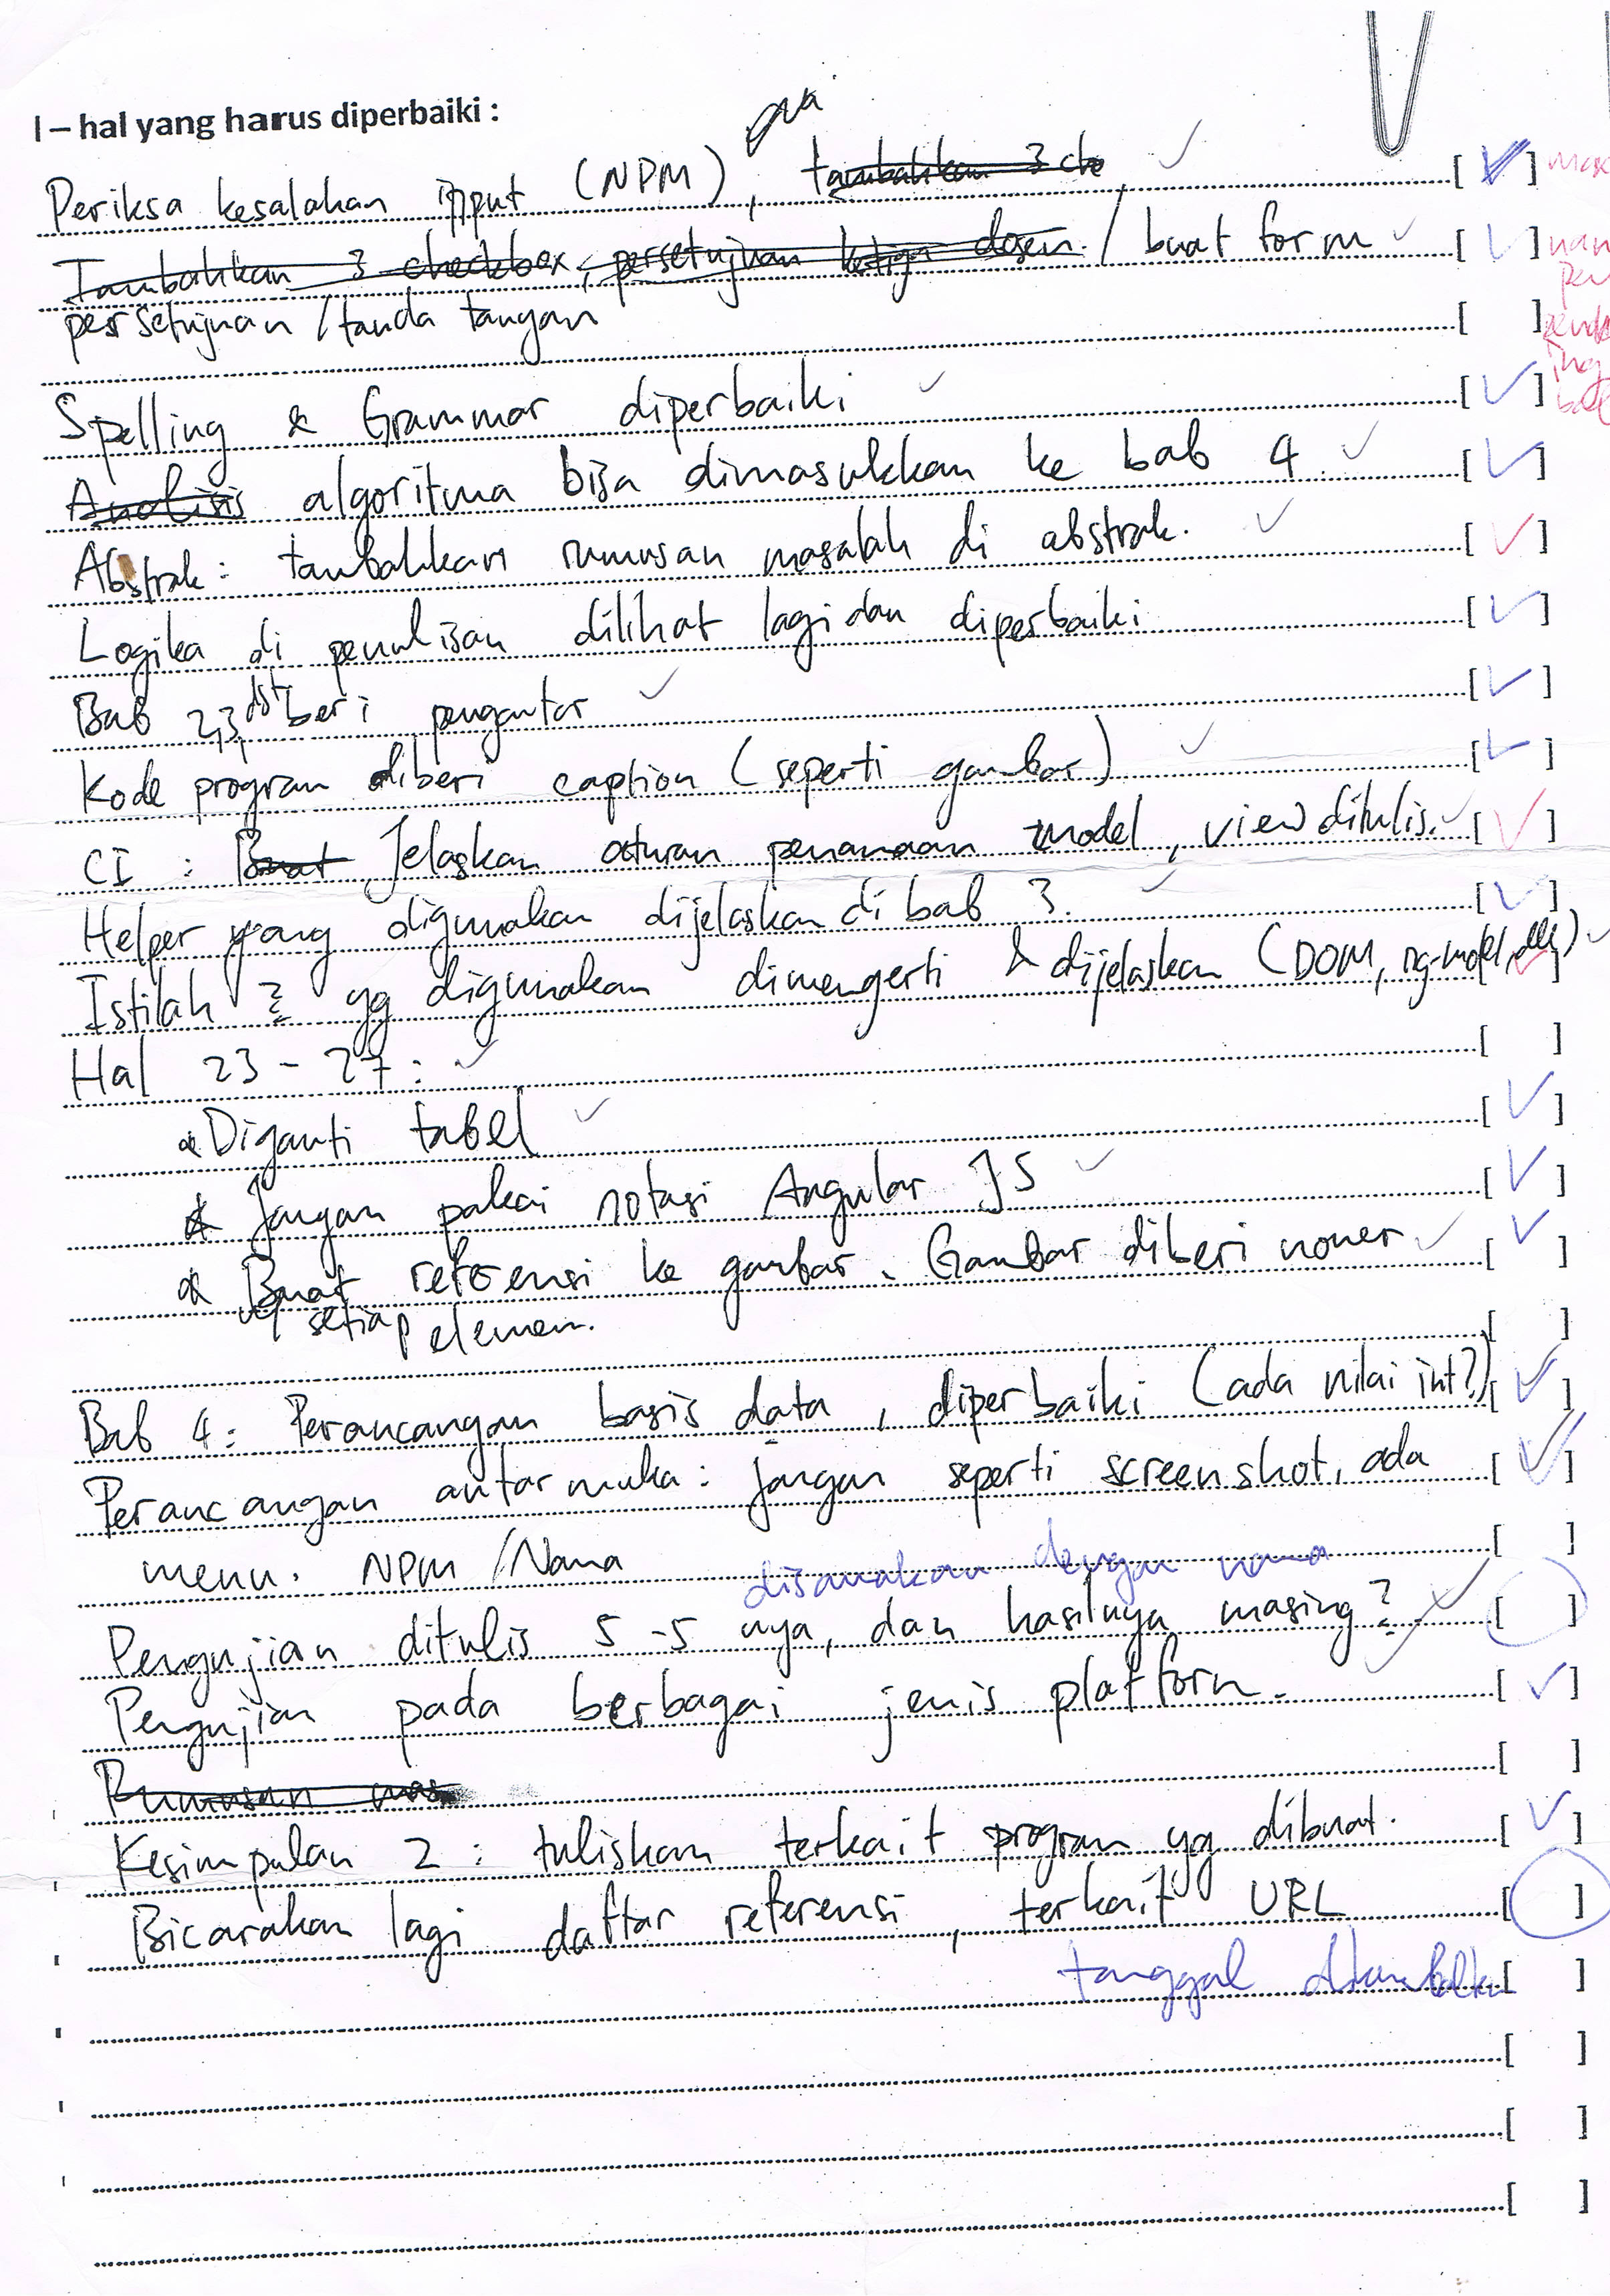
\includegraphics[scale=0.60]{Gambar/revisi}
\caption[Form Revisi Skripsi]{Form Revisi Skripsi} 
\label{fig: revisi}
\end{figure}
}{}
\ifdefstring{\vlmpd}{1}{\include{Lampiran/lampD}}{}
\ifdefstring{\vlmpe}{1}{\include{Lampiran/lampE}}{}
\ifdefstring{\vlmpf}{1}{\include{Lampiran/lampF}}{}
\ifdefstring{\vlmpg}{1}{\include{Lampiran/lampG}}{}
\ifdefstring{\vlmph}{1}{\include{Lampiran/lampH}}{}
\ifdefstring{\vlmpi}{1}{\include{Lampiran/lampI}}{}

\end{document}
